\documentclass[14pt,a4paper,oneside]{article}

\usepackage[utf8]{inputenc}   


\usepackage{amsmath,amsthm,amssymb,appendix,bm,mathrsfs,ctex,geometry,tcolorbox,fancyhdr,tikz,esint}


%% GB/T 7714 宏包 ---- 引文格式
\usepackage[sort&compress]{gbt7714}
\bibliographystyle{gbt7714-numerical}



\numberwithin{equation}{subsection}             %%%%%% 公式编号




\geometry{left=1.7cm, right=1.7cm, top=2.54cm, bottom=2.54cm}    %%%%% 页面尺寸
\linespread{1.5}                             %%%%% 行距1.5倍
\pagestyle{fancy}



%%    设置页眉页脚
\fancyhf{}
\renewcommand{\headrulewidth}{0.15mm}
\fancyhead[C]{文献阅读报告}                   %%%%%% 页眉
\fancyfoot[C]{\thepage}                      %%%%%% 页脚 页码
\setlength{\headheight}{15pt}


%%   设置各种链接颜色为黑色
\usepackage[colorlinks,
            linkcolor=black,
            anchorcolor=black,
            citecolor=black,
            urlcolor=black
            ]{hyperref}



%%   例子编号
\newcounter{example}
\counterwithin{example}{subsection}
\newcommand{\examplename}{Example}
\newcommand{\exampleTitle}[1]{%
\textbf{\refstepcounter{example}\examplename\theexample:#1}\par}


%%  插入图片配置
\usepackage{graphicx,subfigure}
\usepackage[]{caption2} %新增调用的宏包
\numberwithin{figure}{subsection}               %%%%%% 图片编号

\graphicspath{ {./Figure/} }            %%%%% 设置图片文件所在目录
\DeclareGraphicsExtensions{.pdf,.svg,.jpeg,.png,.jpg}     %%%%% 支持图片格式


%%    支持tikz作图
\usepackage{tikz}
\usetikzlibrary{backgrounds,arrows}


\usepackage{pgfplots}
\pgfplotsset{compat=1.15}
\usepackage{mathrsfs}


\title{\textbf{文献阅读报告 1}\\\textbf{High-energy few-cycle pulses: post-compression techniques}}                              %%%%% 标题
\author{骆禹天}                                           %%%%% 作者
\date{2024/**/**}                                        %%%%%% 日期

%%   定义一些数学格式
\newtheorem{theorem}{定理}[subsection]
\newtheorem{definition}[theorem]{定义}
\newtheorem{lemma}[theorem]{引理}
\newtheorem{corollary}[theorem]{推论}
\newtheorem{example}[theorem]{例}
\newtheorem{proposition}[theorem]{命题}
\renewcommand{\abstractname}{\Large\textbf{摘要}}




%%%%%%%%%%%%%%%%%%%% 开始文档  %%%%%%%%%%%%%%%%%%%%%



\begin{document}


\pagenumbering{Roman}         %%%%% 目录前页码统计按罗马数字

\maketitle

\setcounter{page}{1}          %%%%% 标题开始统计页数

%%%%%%%%%%%%%%%%%%%% 目录  %%%%%%%%%%%%%%%%%%%%%

\tableofcontents              %%%%% 插入目录

\newpage                      
\setcounter{page}{1}          %%%%% 目录后重新统计页数


\pagenumbering{arabic}        %%%%% 目录后统计页码为阿拉伯数字



%%%%%%%%%%%%%%%%%%%% 开始第一节  %%%%%%%%%%%%%%%%%%%%%




\section{Introduction}

当代超快科学需要可靠的高能少周期的光脉冲，目前有两种方法生成：短激光脉冲的后压缩和光学参量啁啾脉冲放大（OPCPA）。本文作者全面地总结了基于克尔效应或电离的后压缩技术, 讨论了后压缩技术的相关类型，包括：散装材料中的自由传播、多板连续体生成、多通道电池、长丝、光子晶体光纤、空心光纤和自压缩技术，并进行了比较分析和展望。

一个脉冲可分别在时域或频域中被完整描述。根据带宽定理（类似不确定关系），两种形式下的宽度乘积有最小值：
\begin{equation}
    \Delta t\cdot\Delta \omega\geq\mathrm{const}
    \label{eq:1.0.1}
\end{equation}

取等号情形称变换极限，代表频谱所有分量同相并相长叠加。少周期超短脉冲的生成要求谱宽应足够宽。由于放大介质的能级宽度有限，多数常用激光器的增益带宽太窄。目前有两种解决方法：

1.后压缩：先展宽脉冲的频谱，再将其压缩到几个周期的持续时间。

2.光参量啁啾脉冲放大（OPCPA）：寻找具有足够增益带宽的介质。涉及虚能态的光学参数过程可以支持任意宽的光谱范围，只有相位匹配条件以及放大介质的光谱传输范围对带宽构成限制。

后压缩包含两个步骤：1.光谱展宽；2.啁啾管理。

根据脉冲持续时间、带宽和中心波长，啁啾脉冲管理有不同的选项。多数后压缩器包含一对啁啾反射镜和一对玻璃楔子，用于连续调节啁啾。为了实现亚 1.5 周期脉冲需要非常精确的啁啾补偿，除啁啾镜外，还可以将具有不同的群延迟色散 (GDD) 与三阶色散比率的块材组合使用，从而合并三阶色散 (TOD)。其他技术还包括脉冲整形器或脉冲合成器，将超宽带频谱首先分成频谱分支，再由不同的啁啾镜分别压缩，最后重新组合。在材料色散改变符号的红外光谱范围内，可以通过在大块玻璃中简单地传播从而取代啁啾镜。

产生光谱展宽的非线性相互作用是由光学克尔效应产生的自相位调制。自相位调制也可由其他非线性效应引起，如光电离。

\section{光谱展宽}

一个电场：$E\left(t,z\right)=a\left(t,z\right)\cos{\left[\phi\left(t,z\right)\right]}$ ，可分为波包 $a\left(t,z\right)$ 以及相位项 $\phi\left(t,z\right)=\omega_0t-k_0z=\omega_0t-z\omega_0n/c$。定义瞬时频率为相位项的时间导数
\begin{equation}
    \omega_{\mathrm{inst}}\left(t,z\right)\equiv\frac{\partial\phi}{\partial t}=\omega_0-\frac{\omega_0}{c}\frac{\partial n\left(t,z\right)}{\partial t}z
    \label{eq:2.0.1}
\end{equation}
光脉冲改变介质折射率，使瞬时频率发生变化，新光谱成分产生光谱展宽。如果折射率变化由脉冲本身引起，称为自相位调制（SPM），如果由另一脉冲引起，称为交叉相位调制（XPM）。多数后压缩使用 SPM。实现这种快速的相位调制有两种物理机制：光克尔效应和光电离。

\subsection{基于光克尔效应的光谱展宽}

如果在介质中传播的光脉冲强度足够高，足以显著地扭曲介质成分的原子势场，价电子在电磁场中会非简谐地振荡，从而改变介质的宏观特性。折射率与电磁场强度相关，称为光克尔效应：
\begin{equation}
    n=n_0+n_2I\left(t,z\right)
    \label{eq:2.0.2}
\end{equation}
其中， $n_0$ 为线性折射率，$n_2$ 为非线性折射率，单位为：$\mathrm{cm^2/W}$ ，I为光强。气体中，非线性折射率与气压成线性关系：$n_2=p\cdot\kappa_2$。瞬时频率为：
\begin{equation}
    \omega_{inst}\left(t,z\right)=\omega_0-\frac{\omega_0}{c}n_2\frac{\partial I\left(t,z\right)}{\partial t}z\
    \label{eq:2.0.3}
\end{equation}

由上式可见：在脉冲包络的斜率上，会创建新的频谱分量，且随着斜率的变化，瞬时频率会发生变化，如图 \ref{p2.1.1} 所示:

\begin{figure}[h]
    \centering
    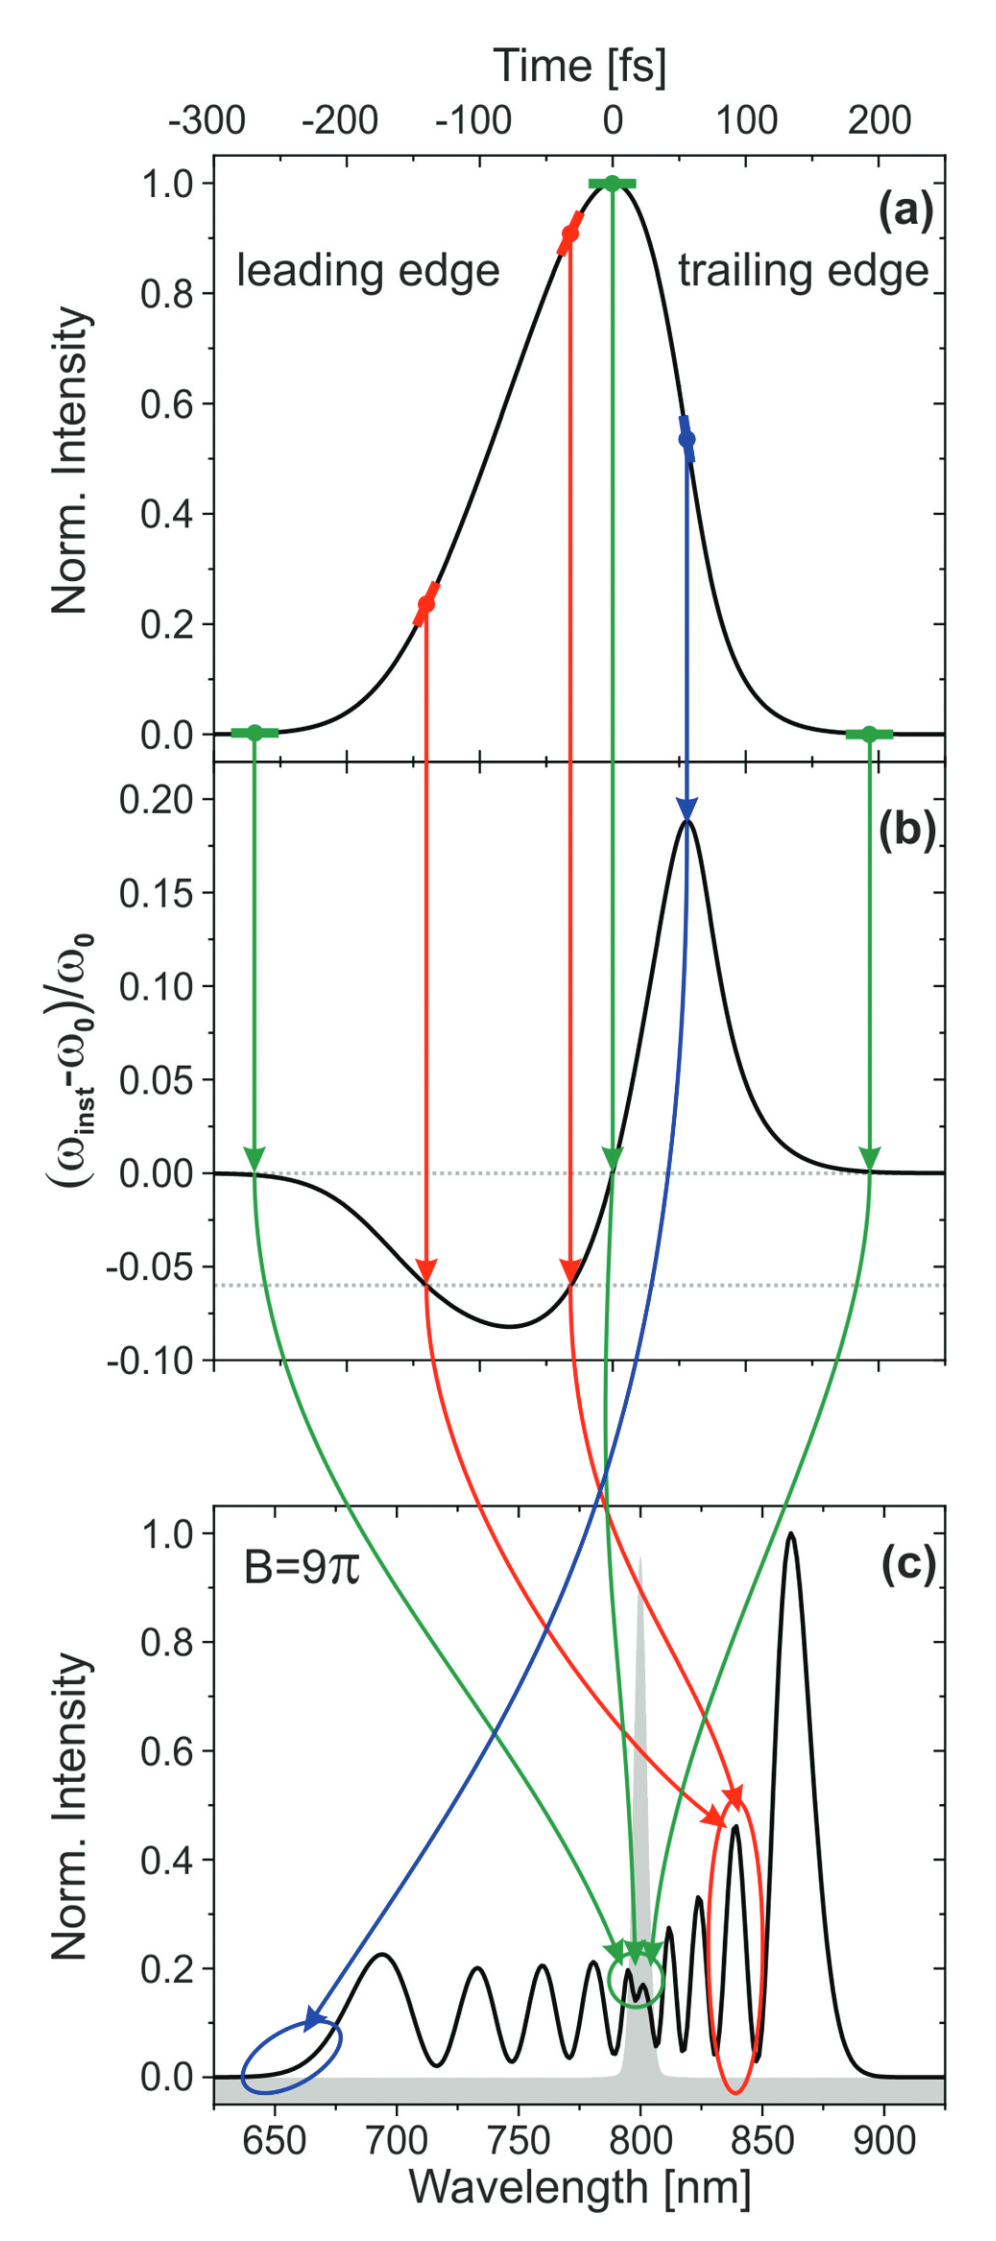
\includegraphics[width=0.3\textwidth]{p1.png}
    \caption{光克尔效应产生自相位调制： (a) 输入脉冲形状；(b) 归一化瞬时角频移；(c) B 积分为 9$\pi$ 处的 SPM 频谱（输入频谱由阴影标记）}\label{p2.1.1}
\end{figure}

如图 \ref{p2.1.1}：

(i) 脉冲前沿使红色侧变宽，后沿使蓝色侧变宽。 

(ii) 光谱两侧的最大位移以及展宽总量由脉冲斜率最大值（蓝线）决定。脉冲较陡部分的光谱的幅度会随着脉冲陡度的增加而迅速地减小。

(iii) 在拐点两侧总有两个位置具相同斜率，生成相同的光谱成分，导致光谱干扰。随时间，光谱条纹周期向中心波长减小。实际上，SPM 展宽的光谱显示出许多 $B/\pi$ 峰。 

(iv) 脉冲峰值和低强度基座处区域贡献中心波长（绿线）周围的光谱。但如果脉冲基座很大会导致中心波长附近出现大幅度的快速振荡。应用时间对比度增强方法（例如非线性椭圆偏振旋转）于未压缩的 SPM 展宽脉冲，可分离脉冲的底座，产生钟形光谱。

克尔效应的影响可通过脉冲峰值处累积的相移 $\varphi$ 的非线性部分来描述，用所谓 B 积分表示：
\begin{equation}
    B=\frac{\omega_0}{c}\int_{0}^{L}{n_2\left(z\right)I\left(z\right)dz}=\frac{2\pi}{\lambda}n_2I_0L_{\mathrm{eff}}
    \label{eq:2.1.3}
\end{equation}

其中，$\ L_{\mathrm{eff}}=\int_{0}^{L}{n_2\left(z\right)/n_2}\cdot I\left(z\right)/I_0dz$ 为非线性相互作用的有效长度，其考虑了传播过程中的强度变化，如损耗或增益的变化以及非线性的变化，如气压变化。高斯脉冲光谱展宽和 B 积分间有如下关系：
\begin{equation}
    F\equiv \Delta\omega_{\mathrm{out}}\Delta\omega_{\mathrm{in}}=\sqrt{1+\frac{4}{3\sqrt{3}}B^2}
    \label{eq:2.1.4}
\end{equation}

其中，F为谱展宽因子，$\mathrm{\Delta}\omega_{in}$ 和 $\mathrm{\Delta}\omega_{out}$ 是非线性相互作用前后脉冲光谱的均方根宽度。如果 B 积分超过 2.5，则光谱展宽因子与 B 积分近似成线性比例：$\mathrm{F}\approx0.88\mathrm{B}$。
钟形空间分布（如高斯分布）的强脉冲在克尔介质中传播，在光斑中心积累最大的相移，越外围相移减小，光斑“聚焦”，类似于通过一凸透镜，这种效应称自聚焦。自聚焦与衍射会产生一个球面波曲率，其平方反比于光束尺寸，因此实际控制传播行为的不是脉冲强度而是峰值功率。如果峰值功率达到自聚焦临界功率（$P_{cr}$），两种效应相互平衡，光束尺寸在传播过程中保持恒定，超过该阈值光束将被聚焦。
\begin{equation}
    P_{\mathrm{cr}}=\frac{1}{2\pi}\frac{\lambda^2}{n_0n_2}
    \label{eq:2.1.5}
\end{equation}

\subsection{气体中光电离引起光谱展宽}

光电离也可导致 SPM。电离过程中产生的自由电子等离子体的折射率小于 1：
\begin{equation}
    n_p=\sqrt{1-\frac{\omega_p^2}{\omega_0^2}}\approx1-\frac{\omega_p^2}{2\omega_0^2},\quad\text{where},\quad \omega_p^2=\frac{e^2}{m_e\epsilon_0}
    \label{eq:2.2.1}
\end{equation}

这里， $\omega_p$ 表示等离子体频率，$\rho$ 是自由电子数密度。气体的折射率接近 1，自由电子引起的折射率变化为：
\begin{equation}
    \Delta n\approx-\frac{\omega_p^2}{2ω_0^2}=-\frac{e^2}{2m_e\epsilon_0\omega_0^2}\rho(t,z)\
    \label{eq:2.2.2}
\end{equation}

离子的复合时间至少为皮秒量级，远长于激光脉冲的持续时间，因此脉冲持续时间内的电子密度为单调递增的阶梯函数。此外，电子密度的动力学演化可很好地通过速率方程描述，在弱电离情形可以进一步简化：
\begin{equation}
    \frac{\mathrm{d}\rho}{\mathrm{d}t}=\omega (\rho_0-\rho)\approx\omega\rho_0
    \label{eq:2.2.3}
\end{equation}

其中，$\rho_0$ 为气体的粒子数密度，$\omega$ 为电离率，它是光强度的非线性函数。联立方程 \ref{eq:2.0.1}、\ref{eq:2.2.2} 和 \ref{eq:2.2.3}，可得到电离情况下的瞬时频率：
\begin{equation}
    \omega_\mathrm{inst}(t,z)\approx\omega_0+\frac{\rho_{0}e^2}{2m_e\epsilon_0c\omega_0}\omega [I(t)]z
    \label{2.2.4}
\end{equation}

上式表明，新产生的频谱分量总是频率高于载波，电离展宽光谱的重心相较输入蓝移。此外，由于电离率和瞬时频率是时间相关的尖锐的钟形函数，因此引入的啁啾信号将具有显著的高阶成分，这使得啁啾管理更加困难。

\section{非线性介质中传播产生光谱展宽}

在均匀非线性介质中传播是最简单的光谱展宽方法。但这存在两个问题：

(i) 由于光谱展宽与 B 积分成正比，如果强度不均匀可能导致光束形状的变化。

（ii）如果脉冲的峰值功率高于自聚焦阈值，自聚焦会导致B 积分超过 ~3。这只能通过将非线性传播分多次进行来缓解。

\subsection{固体介质中自由传播}

1988年， C. Rolland 和 P. B. Corkum 在体介质中进行光谱展宽并利用光栅对压缩脉冲，如图\ref{p3.1.1}所示，实现了 7-110 $\mathrm{\mu J}$， 19-24 fs 的脉冲，代表了该时间尺度上的能量记录。\cite{rollandCompressionHighpowerOptical}

\begin{figure}[h]
    \centering
    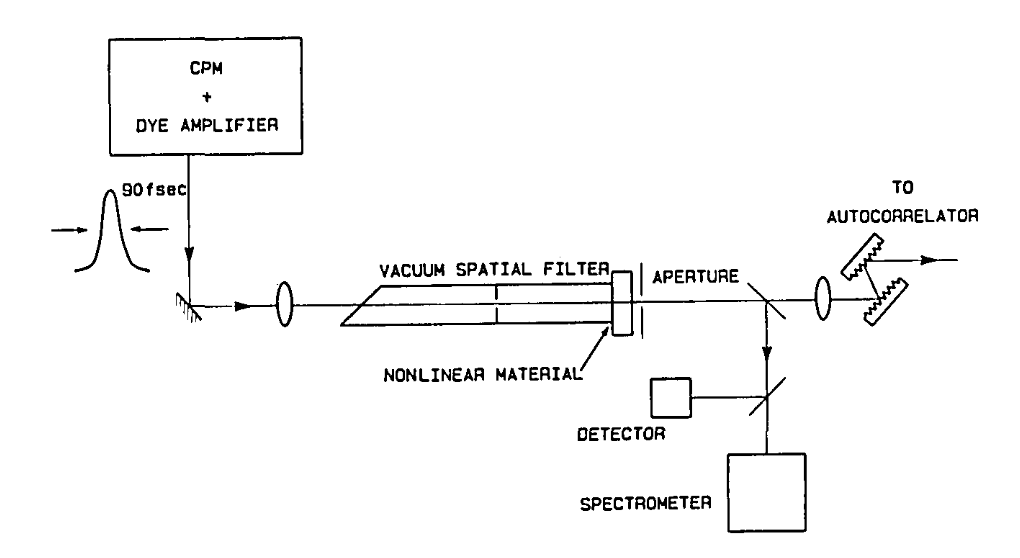
\includegraphics[width=0.5\textwidth]{p2.png}
    \caption{C. Rolland 和 P. B. Corkum应用固体介质实现光谱展宽\cite{rollandCompressionHighpowerOptical}}\label{p3.1.1}
\end{figure}

然而上面配置中，光谱的一致性需要取舍，体介质后的空间滤波器用于选择光束的中心部分，其中 SPM 是空间均匀的。如果选择的空间滤波孔径远小于光束直径，这种近场空间过滤便能产生空间均匀的光束。然而，这将后压缩系统的透过率限制在百分之几。 在此基础上，E. Me ́vel等人改进了C. Rolland 和 P. B. Corkum 的设置，如图 \ref{p3.1.2} 所示，并实现 70 $\mathrm{\mu J}$  ， 12 fs 的脉冲以及 220 $\mathrm{\mu J}$  ， 14 fs 的脉冲。\cite{mevelExtracavityCompressionTechnique2003}

\begin{figure}[h]
    \centering
    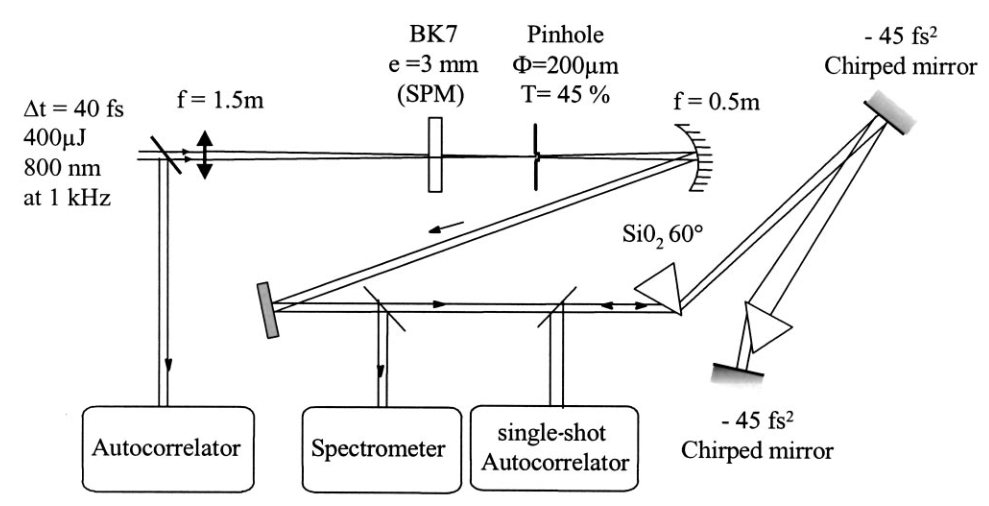
\includegraphics[width=0.4\textwidth]{p3.png}
    \caption{E. Me ́vel等人的改进配置\cite{mevelExtracavityCompressionTechnique2003}}\label{p3.1.2}
\end{figure}

使用薄膜压缩 (Thin Film Compression,TFC)的方法， G. Mourou 等人设想在模拟的基础上，使用约 500 $\mathrm{\mu m}$  、直径 20 cm 的“塑料”薄膜，薄膜对激光波长透明、能保持坚固与柔韧且具有均匀厚度，从而生成单周期 100 J 量级的脉冲以及 $1024 \mathrm{W/cm^2}$ 的超相对论强度。\cite{mourouSingleCycleThin2014}

\begin{figure}[h]
    \centering
    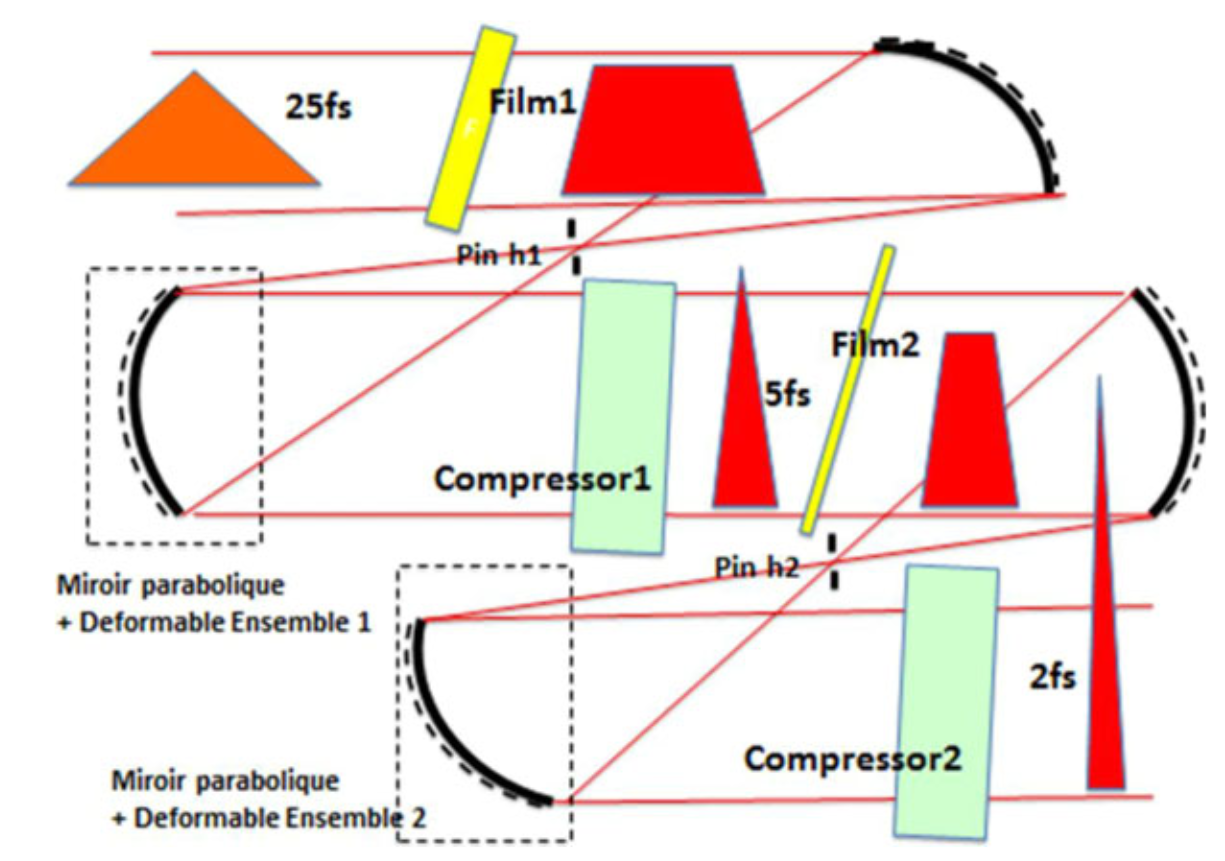
\includegraphics[width=0.32\textwidth]{p4.png}
    \caption{TPC 示意图\cite{mourouSingleCycleThin2014}}\label{p3.1.3}
\end{figure}

TPC 如图\ref{p3.1.3}所示，激光束通过约为 10 的离轴抛面镜聚焦。聚焦光束有两个作用： 

a) 通过小范围上下滑动薄膜优化光束强度；

b) 提供一种消除由小规模自聚焦引起光束不均匀的方法。接着，在焦点处放置适当尺寸的光阑，然后光束的焦点通过第二个抛面镜重新成像到无穷远，再使用标准单次自相关技术来测量脉冲。

下一节中的模拟演示了在初始阶段使用 500 $\mathrm{\mu m}$厚的薄膜将 27 J、27 fs 的脉冲压缩至 6 fs 的可能性。第二级的塑料厚度为 100 $\mathrm{\mu m}$，进一步将脉冲压缩至 2 fs。

如图 \ref{p3.1.4} 所示的模拟所示，光束经压缩后仍保持良好的质量。然而目前 TPC实现目标仍遥远，但在适度的压缩因子下已在能量扩展方面取得了实质进展。

\begin{figure}[h]
    \centering
    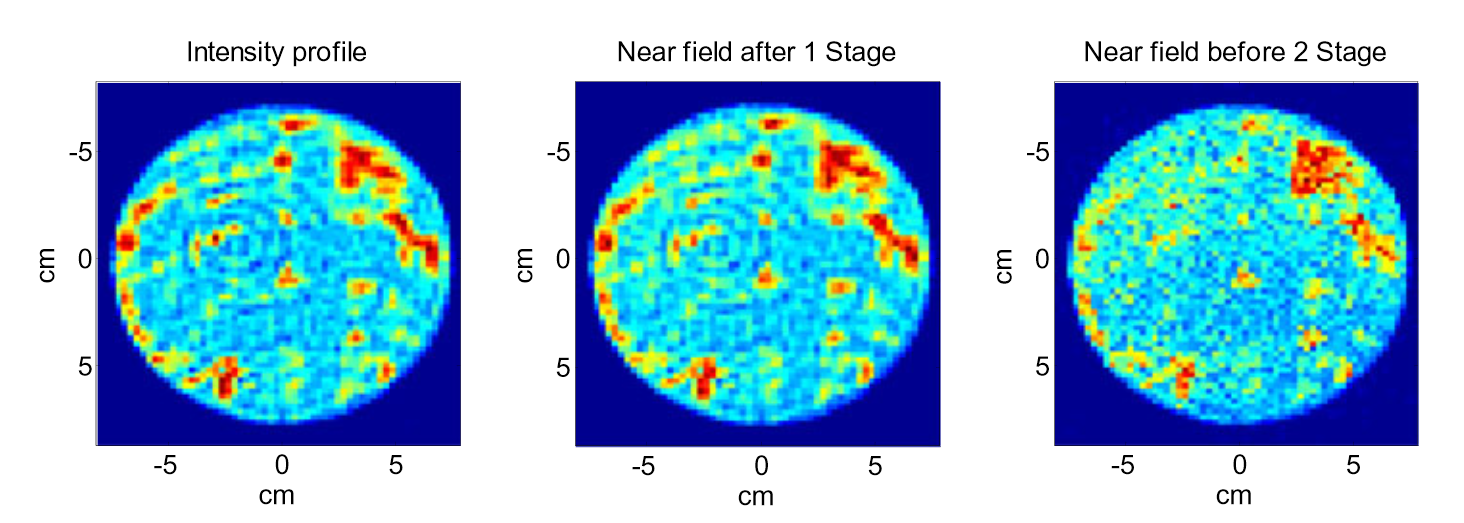
\includegraphics[width=0.6\textwidth]{p5.png}
    \caption{TPC 产生光束轮廓上的强度分布：a) 激光输出处，b) 第一级之后（无空间滤波器），c) 第二级之后（无空间滤波器）。\cite{mourouSingleCycleThin2014}}\label{p3.1.4}
\end{figure}

\subsection{多板连续生成 Multiple-plate continuum generation}

A.H.Kung等人将非常薄（0.1–0.5 mm）的玻璃板放置在强度约 20 $\mathrm{TW/cm^2}$ 的强会聚光束中，如图 \ref{p3.2.1} 所示。峰值功率比玻璃板的临界功率大几百倍，光束自聚焦，但玻璃板非常薄，光束在坍塌前已经离开玻璃板，并在玻璃板后方的空气中聚焦。在焦点后，放置另一个玻璃板，发散光束在下一个玻璃板内部自聚焦而重新聚焦。每个板可引入4–5的B积分，一系列这样的聚焦薄板可以产生 450 - 980 nm 超过一个倍频程的超连续谱（图\ref{p3.2.1}（b））和非常大的压缩因子，直至单循环极限。\cite{luGenerationIntenseSupercontinuum2014}

\begin{figure}[h]
    \centering
    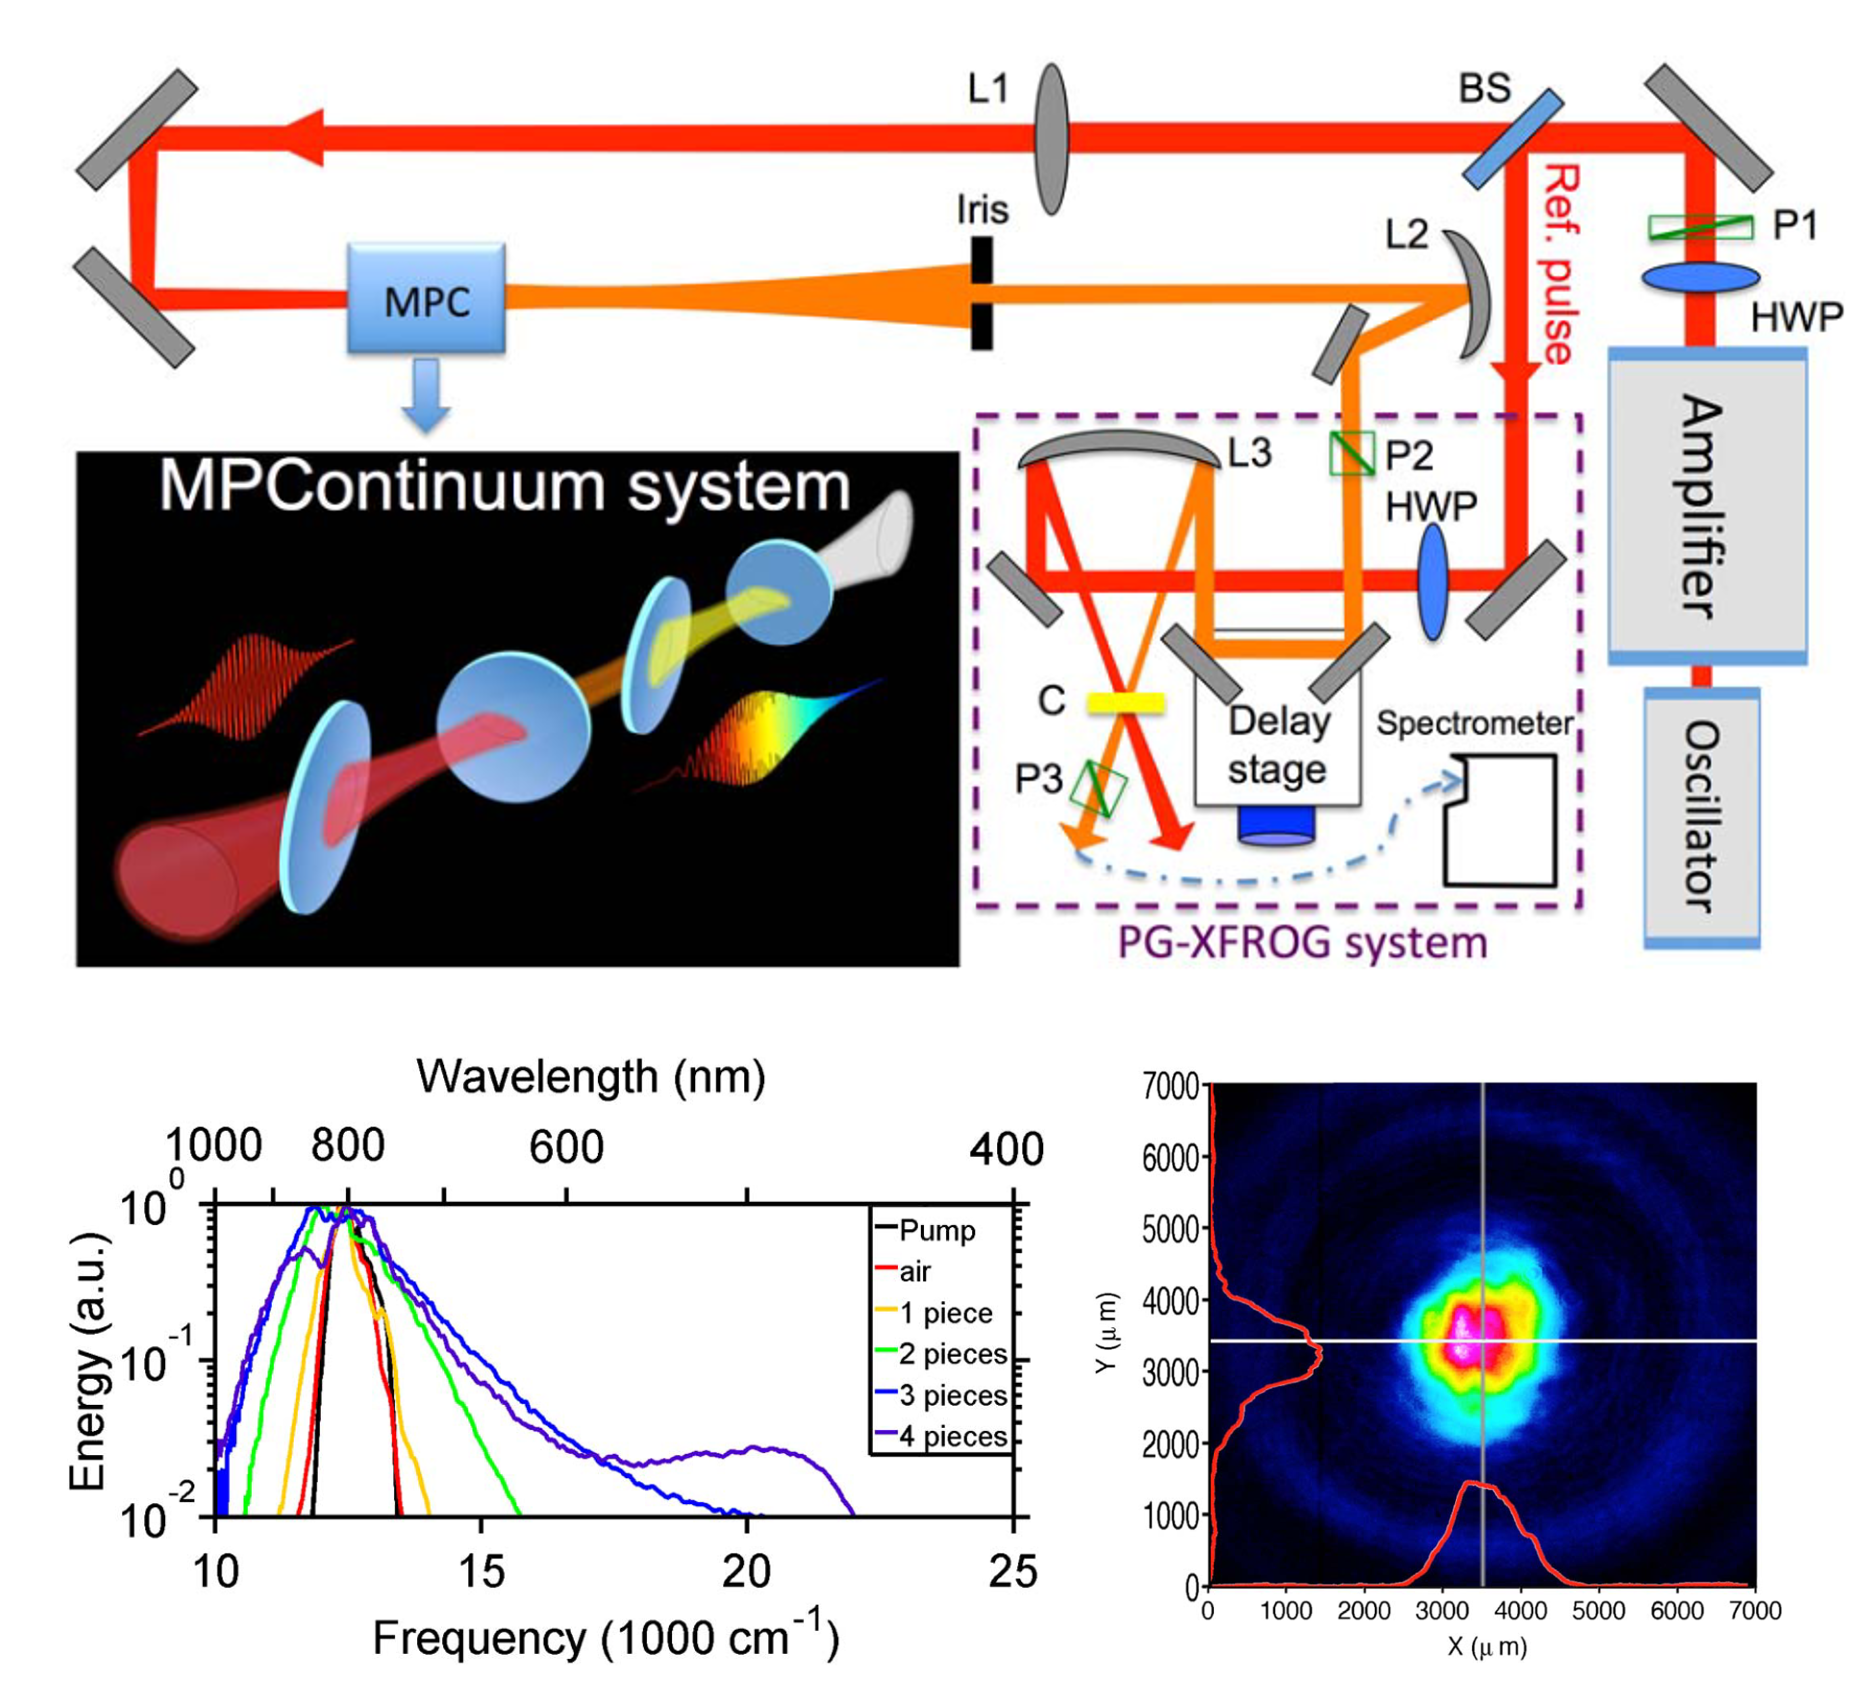
\includegraphics[width=0.4\textwidth]{p6.png}
    \caption{（a）多板连续生成的示意图；（b）输入光谱以及仅经过空气和经过一定数量玻璃板后的加宽光谱；（c）CCD表征输出光斑\cite{luGenerationIntenseSupercontinuum2014}}\label{p3.2.1}
\end{figure}

该技术缺点是能量可扩展性较差（亚 mJ 状态），因为其依赖材料自身的非线性产生自聚焦，并且应用这种方法输出光束剩余的空间啁啾很少。\cite{luSub4FsLaser2018}

\subsection{多通腔 （MPC）}

多通腔与之前的方法类似，非线性相互作用发生在焦点附近。但多通腔中，重新聚焦通过光学器件实现而非非线性效应的自聚焦。多通腔中，非线性介质被放置在赫里奥特型腔内，该腔保留了光束参数并充当“离散”波导（图 \ref{p3.3.1} （a））。在这样的腔体中，即使每次通过非线性介质只产生较低的非线性效应（$B\ll pi$），但经过几十次往返通过非线性介质后可以累计大量的光谱展宽，如图 \ref{p3.3.1} (b) 所示。

\begin{figure}[h]
    \centering
    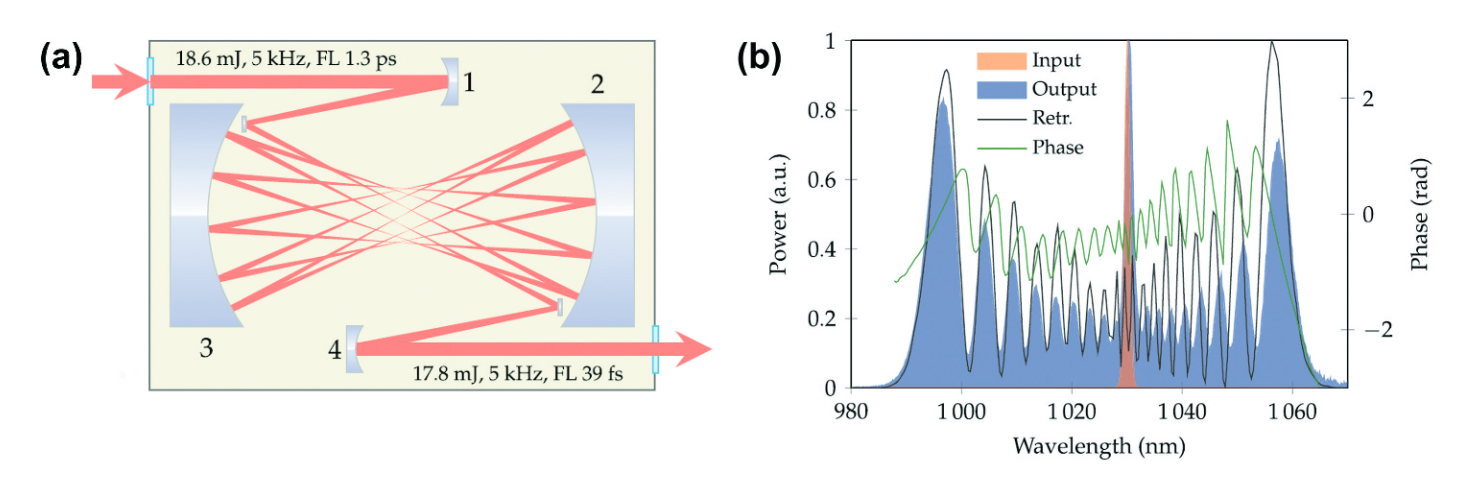
\includegraphics[width=0.8\textwidth]{p7.png}
    \caption{ （a）多通腔示意图；（b）多通腔实现光谱展宽\cite{kaumannsMultipassSpectralBroadening2018}}\label{p3.3.1}
\end{figure}

多通腔优点：

1.单次通过下，较低B 积分可以保持光束参数稳定以及腔体匹配。

2.自由空间传播分离了克尔非线性，导致整个光束轮廓上的光谱均匀分布。

3.非线性材料的丰富选取：最初，多通腔采用玻璃作为较低能量（$\mathrm{\mu J}$量级）下的非线性介质，后来为提高脉冲能量至毫焦量级，赫里奥特腔被密封并充入惰性气体代替固体作为非线性介质。

4.压缩至短的持续时间：大多数结果都报告了压缩持续时间不短于约 20 fs。

5.高能量，高平均功率，高效率：多通腔压缩器专为高重复率、高功率的板条和薄盘激光器开发，可提供持续时间 100 fs 量级至 ps 量级的脉冲，其效率约为 85\% -95\% 具体取决于腔镜的反射率和往返次数。

Martin Kaummans等人使用单级充气多通腔，在充满 600 mbar 氩气的 45 通腔内，将一个持续时间为 1.3 ps，能量为迄今为止最高的 18 mJ 的脉冲在平均功率为 90 W 的情况下压缩至 41 fs（图 3.3.1（a）），这一结果的压缩系数达到了创纪录的约 32，且整体传输率高达 95.7\% 。\cite{kaumannsMultipassSpectralBroadening2018}

P Russbueldt 等人利用MPC技术，还在 44 通腔内以 500 kHz 重复率将 590 fs ，1.1 mJ 的脉冲压缩至 30 fs（20 倍压缩），实现了 530 W 的最高平均功率，效率为 96\% 。\cite{russbueldtScalable30Fs2019}

\subsection{成丝（Filament）}

如果超短脉冲在透明介质中传播的峰值功率超过自聚焦临界功率数倍（5-10倍），就会发生自引导传播，称为成丝。它主要来源于克尔效应（自聚焦、SPM 和自陡峭）、光电离（吸收和散焦）和线性效应（衍射和色散）之间复杂的相互作用，达到一种动态平衡，使激光脉冲在介质中形成很长的，较稳定的激光通道。成丝传播过程中，脉冲光谱不对称展宽，蓝色一侧出现又长又弱的拖尾（见图\ref{p2.1.1}），其主要由涉及强自陡峭的光克尔效应造成。\cite{couaironFemtosecondFilamentationTransparent2007, bergeUltrashortFilamentsLight2007, gaetaCatastrophicCollapseUltrashort2000}

成丝在固体、液体和气体中，由于的不同线性和非线性性质，强度非常不同。

固体中，成丝是由μJ量级低能量fs到ps脉冲引起的。这一过程导致相干白光或超连续谱的产生，频率跨越几个八度（倍频），光谱密度约为10 pJ/nm。成丝技术简单稳健，在光谱学，光源领域中有许多应用，例如通过催化OPCPA系统。

气体中，在mJ量级脉冲能量下发生成丝现象。

相关研究：

U.Keller首先在钛宝石激光脉冲压缩中利用成丝现象。\cite{hauriGenerationIntenseCarrierenvelope2004}

C.P.Hauri等人在两个级联氩丝中展宽光谱，获得了能量为0.38mJ、5.7fs、CEP稳定的脉冲。后来，该组逐渐将脉冲压缩至5.1 fs，最终到4.9 fs。\cite{hauriGenerationIntenseFewcycle2005, zairSpatiotemporalCharacterizationFewcycle2007}

使用2周期脉冲作为成丝的输入，在氩\cite{akozbekExtendingSupercontinuumSpectrum2006}和氦\cite{goulielmakisUltrabroadbandCoherentLight2008}中获得了能量高达200$\mathrm{\mu J}$，光谱范围从低于300 nm到超过1μm。

M.Kovacev组通过使用35fs输入脉冲在充满氩气的气体腔中诱导单根细丝，获得了7fs脉冲和随后的亚4fs脉冲。通过改变灯丝后啁啾镜引入的啁啾，他们在几个啁啾设置下观察到压缩脉冲，这表明脉冲结构相当复杂。\cite{steingrubeSub15cyclePulsesSingle2012}

800nm波长激光脉冲驱动成丝存在严重的能量限制，可以通过放大激光波长和匹配传播过程几何结构来缓解。因此，在中红外光谱范围内可以获得更高的脉冲能量，这主要是由于临界功率下的波长缩放。\cite{heylScaleinvariantNonlinearOptics2016, zheltikovLaserinducedFilamentsMidinfrared2017}

然而，大多数组已放弃利用成丝作用在可见光/近红外范围进行后压缩，主要原因是：在光丝中，时间脉冲轮廓随着光束轮廓中仅在中心具有最佳形状的横向位置而变化很大。因此，只有光束的中心区域，包含远低于1mJ的一小部分全能量，可用作短脉冲源。

除光谱展宽外，成丝过程中丰富的动力学还可以导致自压缩。

\section{波导中的光谱展宽}

使用波导展宽光谱相对在自由空间中传播可解决两个基本问题：

（i）波导中，脉冲可在仅由波导几何形状定义的扩展长度上保持其光束大小，从而保持高强度。光束大小可超过聚焦的瑞利长度几个量级，能积累非常大的B积分，增大光谱展宽。

（ii）在波导中传播，光束来回反射相干叠加形成本征模。本征模在整个光束轮廓中无论时域和频域上都表现出相同行为，原则上允许完美的脉冲压缩。此外，考虑到本征模理想（衍射受限）的光束特性，脉冲能量也可以理想地聚焦，从而产生尽可能高的强度。然而，只有当传播中只涉及一个本征模时，这种理想情况才成立，否则不同模式以不同速度传播，导致不可补偿的时间拖尾（模态色散）和恶化的聚焦性质。

减小模式色散的最直接方法是使用只有一种模式能够传播的波导，如采样单模光纤，但压缩脉冲的能量无法太高不能超过几个nJ，导致峰值功率无法达到MW水平，聚焦强度达到$10^{11}–10^{12} \mathrm{W/cm^2}$，从而限制了时间分辨光谱领域的应用。

\subsection{波导中传播的能量和功率范围}

波导中良好控制的脉冲传播有两个主要标准\cite{vozziOptimalSpectralBroadening2005}：

（i）输入脉冲的峰值功率应低于自聚焦的临界功率（$P_0<P_{\mathrm{cr}}$）；

（ii）脉冲的峰值强度应低于非线性介质的电离阈值（$I_0<I_{\mathrm{th}}$）。

这两个标准一方面为了避免损坏波导。另一方面在多模光纤中，自聚焦和光电离中产生的自由电子都会改变光束的发散性，从而导致本征模之间的耦合（模式混合），造成模式色散和损耗增加。

在波导中，每个本征模都有其有效面积$A_{\mathrm{eff}}$，效面积仅取决于模式分布。在传播过程中有效面积与脉冲的峰值功率和峰值强度间有恒定关系：
\begin{equation}
    I_0=\frac{P_0}{A_{\mathrm{eff}}}
    \label{eq:4.1.1}
\end{equation}

根据（i），要在增加输入的峰值功率，需要相应提高自聚焦的阈值功率才能避免自聚焦。由等式\ref{eq:2.1.5}，这要求降低非线性折射率满足不等式：
\begin{equation}
    n_2<\frac1{2\pi}\frac{\lambda^2}{n_0P_0}
    \label{eq:4.1.2}
\end{equation}

代入\ref{eq:2.1.3}，有：
\begin{equation}
    B=\frac{2\pi}\lambda n_2I_0L_{\mathrm{eff}}<\frac\lambda{n_0}\frac{L_{\mathrm{eff}}}{A_{\mathrm{eff}}}
    \label{eq:4.1.3}
\end{equation}

注意，为避免波导中自聚焦，介质中给定中心波长下，可实现的光谱展宽仅受光纤几何形状的限制，而不取决于脉冲的其他参数或介质的性质。

考虑到等式\ref{eq:4.1.1}，为通过放大峰值功率来防止电离，需要增加有效模面积以满足：
\begin{equation}
    A_{\mathrm{eff}}>\frac{P_0}{I_{\mathrm{th}}}
    \label{eq:4.1.4}
\end{equation}

等式\ref{eq:4.1.3}和\ref{eq:4.1.4}可合并为一个关系，其描述了在波导中传播期间的光谱增宽的极限：
\begin{equation}
    B<\frac\lambda{n_0}\frac{I_{\mathrm{th}}}{P_0}L_{\mathrm{eff}}
    \label{eq:4.1.5}
\end{equation}

根据等式\ref{eq:4.1.5}，为了避免由于波导中的自聚焦或电离而导致的模式混合，可实现的最大光谱增宽取决于：

（1）输入脉冲（$\lambda$；$P_0$）；

（2）非线性介质（$n_0$；$I_{\mathrm{th}}$）；

（3）波导几何结构（$L_{\mathrm{eff}}$）。

通常，对给定中心波长，通过放大输入脉冲的峰值功率（并相应地匹配波导的有效面积和非线性折射率），可实现的光谱展宽减小，这只能通过增加非线性相互作用的长度来补偿。对于给定的中心波长，综合上述总结为一个关系：
\begin{equation}
    P_0\propto\frac1{n_2}\propto A_{\mathrm{eff}}\propto L_{\mathrm{eff}}
    \label{eq:4.1.6}
\end{equation}
根据上式，增加脉冲能量有两种方式：

（i）具有大模场面积的单模光纤；

（ii）大孔径的多模波导。

两种方法都以气体作为非线性介质，此外，考虑到临界功率的波长依赖性（见等式\ref{eq:2.1.5}和良好控制的第一个标准（i））以及电离率的波长依赖性，长波范围（例如中红外）可提高能量放大潜力。

\subsection{光子晶体光纤}

P.St.J.Russell课题组发明了光子晶体光纤，如图\ref{p4.2.1}所示。\cite{knightAllsilicaSinglemodeOptical1996}光子晶体光纤中光的传输不是利用高折射率纤芯和低折射率包层间的全内反射，而是通过光子带隙或由包层的周期性结构引起的其他机制实现，其中基模被包层带隙限制，而高阶模不被包层阻挡而泄漏出去。

\begin{figure}[h]
    \centering
    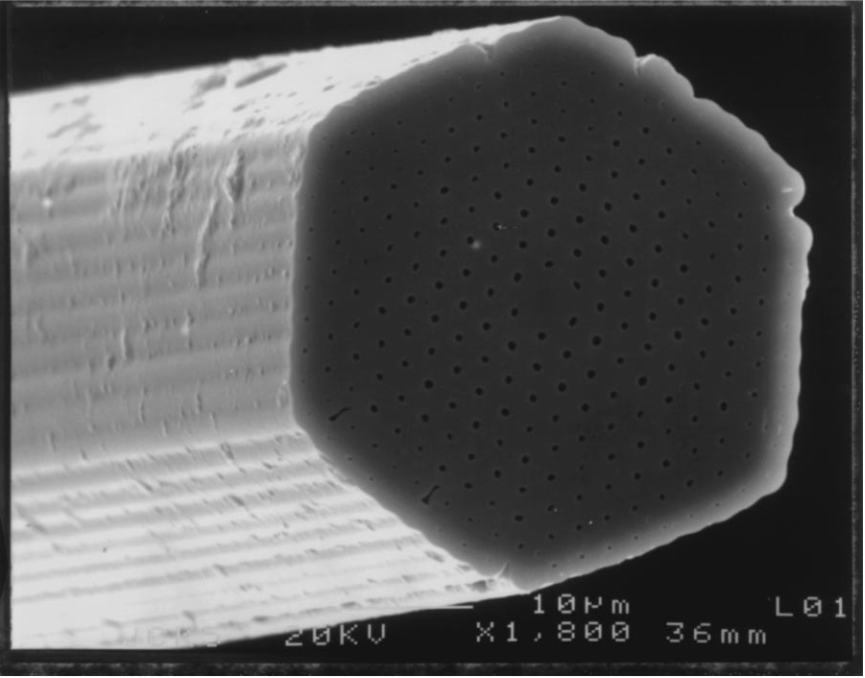
\includegraphics[width=0.25\textwidth]{p8.png}
    \caption{光子晶体光纤的扫描电子显微镜照片\cite{knightAllsilicaSinglemodeOptical1996}}\label{p4.2.1}
\end{figure}

光子晶体光纤的优点：

（1）具有比标准单模二氧化硅光纤更大纤芯尺寸；

（2）适用空心结构（HC-PCF）；\cite{creganSingleModePhotonicBand1999}

（3）色散特性可被设计为匹配预定的光谱色散函数。

光子晶体光纤的问题：光子的带隙只能引导光谱较窄的光，不太适合脉冲压缩。

F.Benabid等人制作了第一个宽带HC-PCF，使用一种称为Kagome晶格的新型包层结构，在近两个倍频程的带宽下实现仅几dB/m的低损耗。这种非常有效的引导机制可以从抑制耦合和反谐振耦合（ARROW）模型的角度得到解释。\cite{benabidStimulatedRamanScattering2002}

\begin{figure}[h]
    \centering
    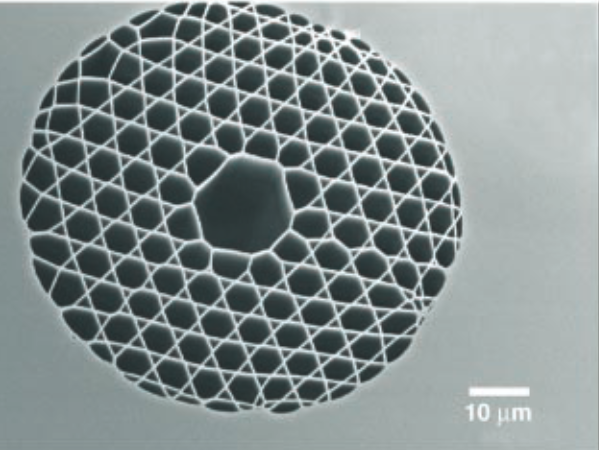
\includegraphics[width=0.25\textwidth]{p9.png}
    \caption{外径为170$\mathrm{\mu m}$的HC-PCF的扫描电子显微镜照片\cite{benabidStimulatedRamanScattering2002}}\label{p4.2.2}
\end{figure}

后来，具有更简单包层结构的负曲率HCF也可以实现类似的性能，例如2011年引入的单环管状晶格光纤。这两种类型的损耗都可以降低到约10 dB/km的水平，以保持宽带运行。\cite{pryamikovDemonstrationWaveguideRegime2011}

如今，基于HC PCF的单模光纤的纤芯尺寸可以达到几十$\mathrm{\mu m}$，乃至创造了超过100$\mathrm{\mu m}$的记录\cite{debordUltraLargeCoreSize2015}，使其适用于平均功率高达100 W、能量为数$\mathrm{\mu J}$的光谱加宽激光脉冲。\cite{emauryEfficientSpectralBroadening2014, kottigGenerationMicrojoulePulses2017}因此，这些波导在亚mJ范围，高功率、高迁移率的系统中有许多应用，如振荡器和光纤激光器\cite{hadrichExploringNewAvenues2015, guichardNonlinearCompressionHigh2015, kottigEfficientSinglecyclePulse2020}。

\subsection{毛细管（Capillaries）或中空芯光纤（Hollow-core fibers）}

1996年，O.Svelto组报告了能量240μJ，10fs脉冲的产生，脉冲能量超出过往几个周期脉冲的能量高出三个数量级。能量提升主要源于两个因素：

（1）气体介质；

（2）大模式面积（式\ref{eq:4.1.6}）。

在此基础上，M.Nisoli等人使用芯径为140 $\mu m$的充气毛细管或空心光纤（HCF）。中空毛细管是弱引导多模波导。由于毛细管的芯部（气体）折射率小于包层（玻璃）折射率，界面上没有全内反射，因此光的传输依赖于掠入射反射，这导致毛细管具有固有的损耗且对弯曲敏感。\cite{marcatiliHollowMetallicDielectric1964}此外，增加模场面积的代价是多模式传输。在这种波导中实现单模传输对脉冲压缩至关重要，需要满足两个条件：

（i）入射脉冲耦合到单个本征模中。需要适当选择聚焦配置使束腰与HCF匹配：$\omega_0\approx0.6436\cdot a$，其中a表示HCF的孔径。\cite{abramsCouplingLossesHollow1972}

（ii）脉冲的全部能量在整个传播过程中保持在这个模式（防止模式混合）。

这些条件与相关技术引入后不久，HCF便允许产生4.5 fs脉冲。\cite{nisoliCompressionHighenergyLaser1997}HCF与色散补偿的啁啾反射镜一起产生了重大影响，对于通过稀有气体中高次谐波过程提供足够强的少周期激励\cite{sartaniaGeneration01TW5fs1997, cerulloFewopticalcycleLaserPulses2000}和高效产生孤立阿秒脉冲\cite{farkasProposalAttosecondLight1992, corkumPlasmaPerspectiveStrong1993, hentschelAttosecondMetrology2001}至关重要。

HCF的优势：

（1）支持高脉冲能量

通过输入~23fs的短脉冲，并保持激光压缩器中较低的非线性，可获得能量0.5mJ亚2周期脉冲\cite{cavalieriIntense5cycleInfrared2007}，随后获得了1mJ能量的脉冲\cite{schweinbergerWaveformcontrolledNearsinglecycleMillijoule2012}。使用圆偏振光可进一步提高能量范围，因为它降低了非线性：圆偏振的非线性折射率是线性情况下的2/3，电离阈值也更高。通过使用圆偏振光和氖作为非线性介质，可以获得1 mJ能量4.3fs的脉冲\cite{chenGeneration43Fs2009}，以及后来能量1.9 mJ但持续时间更长为5.7 fs的脉冲\cite{andersonMultimJCarrierEnvelope2011}。

（2）与光纤激光器匹配

由于具有相似几何形状，HCF压缩器与光纤激光器特别匹配。掺镱光纤激光器发射1030 nm持续时间为几百fs的脉冲，HCF可作为掺镱光纤激光器的自然延伸将脉冲缩短到几个周期。\cite{hadrichHighEnergyUltrashort2009, lavenuHighenergyFewcycleYbdoped2017}由于光纤激光器的平均功率超过了50 W量级，J.Limpert的团队为其光源开发了一种水冷式HCF压缩器，该压缩器能够处理高达kW量级的高平均功率。\cite{hadrichScalabilityComponentsKWlevel2016}在第一项研究中，在93 W的破纪录平均功率下，以1 MHz重复率将700 fs长的0.2 mJ脉冲压缩至81 fs持续时间\cite{rothhardtMHzRepetitionRate2011}。后来，该小组在135 W的平均功率下获得了0.54 mJ、26 fs的脉冲\cite{hadrichNonlinearCompressionSub30fs2013}。在两级级联的布置中，J.Rothhardt等人将150 kHz重复率下的1 mJ、210 fs脉冲压缩为7.8 fs的几个周期持续时间，52.5 W下的能量为0.35 mJ\cite{rothhardt53AveragePower2014}。随后，S.Hädrich等人通过级联HCF设置，以216 W的前所未有的平均功率实现了几个周期6.3 fs脉冲。\cite{hadrichEnergeticSub2cycleLaser2016}该压缩机的第一级以406W的更高功率运行。

（3）支持短波红外和深紫外光谱

在短波红外（SWIR）的较长波长下，使用标准HCFs生成了亚3周期、1425 nm、能量为0.4mJ的脉冲\cite{giguerePulseCompressionSubmillijoule2009}和亚2周期、1.8 $\mu m$脉冲\cite{schmidtCompressionMmLaser2010, schmidtCEPStable162011}。压缩掺铊光纤激光器产生的脉冲，在平均功率超过15 W的情况下，在HCF中获得了7周期2 $\mathrm{\mu m}$脉冲\cite{gebhardtHighAveragePower2017}。HCFs也被用于在深紫外（DUV）中产生超短脉冲。在波长在270 nm的实验中，充气HCF被用于产生和频以及脉冲的光谱加宽\cite{durfeeIntense8fsPulse1999}。用这种方法获得了能量1 $\mathrm{\mu J}$ 的8fs脉冲。随后，我们的小组在HCF中将KrF准分子激光器发射的248nm、100fs脉冲在20$\mu J$能量下压缩到 20fs以下。\cite{steingrubeSub15cyclePulsesSingle2012}

在HCF压缩器在亚mJ的能量水平下饱和。这可通过充气HCFs情况下的缩放定律（等式 \ref{eq:4.1.6}）来解释：
\begin{equation}
    P_0\propto\frac1{p\cdot\kappa_2}\propto a^2\propto L_{\mathrm{eff}}
    \label{eq:4.1.7}
\end{equation}

HCFs的长度实际上限制在约1米，主要原因是：HCFs对弯曲非常敏感，这会导致快速发生模式混合并增加损耗，因此毛细管需要非常直；事实上，平直度是HCFs的主要优点。当时用于压缩的毛细管是厚壁刚性熔融石英管，孔径为200至300 $\mathrm{\mu m}$，外径为1–2 mm。为了保持毛细管平直，将其放入带有V形槽的机械加工支架中，如图\ref{p4.3.1}（a）所示。在这种结构中，合适的光引导被毛细管和V形槽的质量限制在大约1米的长度。在这种情况下HCF中只能使用非线性降低的材料，如氖或氦。\cite{nisoliTerawattscaleSub10fsLaser1998}

\begin{figure}[h]
    \centering
    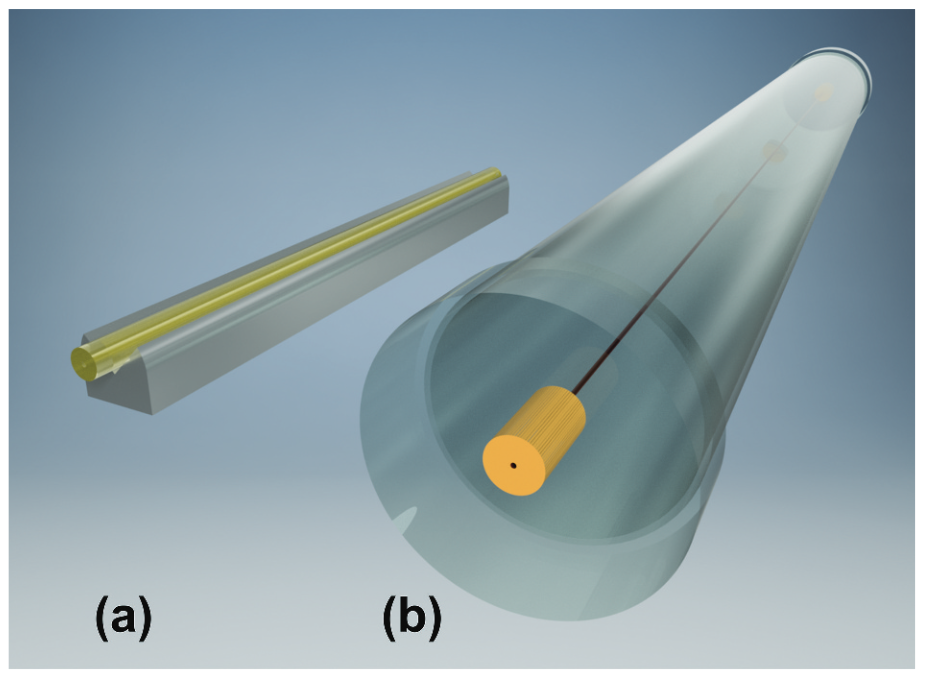
\includegraphics[width=0.3\textwidth]{p12.png}
    \caption{中空纤维：（a）标准毛细管；（b）拉伸的柔性中空芯纤维。\cite{nagyHighenergyFewcyclePulses2021}}\label{p4.3.1}
\end{figure}

这种限制在G. Andriukaitis等人的工作中可以清楚地观察到，G. Andriukaitis等人使用标准HCF在氖中压缩1030 nm、6 mJ、200 fs的长脉冲。虽然获得了4 mJ的压缩脉冲能量；但由于HCF的长度限制，不支持短于35fs的脉冲。

使用在下一节中讨论的方法可以克服HCFs的长度限制，从而扩展到更大的功率范围。

\subsection{拉伸柔性中空芯纤维}

4.1节中提及，要提高能量范围，需要增加有效模场面积，其与孔径a成比例，以及波导长度L。空心波导的传输可以用比尔定律描述：
\begin{equation}
    T=\exp(-\alpha L)
    \label{eq:}
\end{equation}
，其中$\alpha$表示波导损耗，根据文献[30]\cite{marcatiliHollowMetallicDielectric1964}：
\begin{equation}
    \alpha=\alpha_0+\alpha_R,\mathrm{~where~}\alpha_0\propto\dfrac{\lambda^2}{a^3}\mathrm{~and~}\alpha_R\propto\dfrac1{\alpha_0R^2}
    \label{eq:4.4.2}
\end{equation}
其中，$\alpha_0$表示直HCF的损耗系数，$\alpha_R$描述了由于具有恒定曲率半径R的波导弯曲而产生的额外损耗。

由于线性损耗系数与内半径的三次方成反比，因此光纤几何形状的放大伴随着峰值功率的增加导致理想 HCF 传输T的净增加。然而，等式\ref{eq:4.4.2}的最后一部分表明，弯曲损耗与$\alpha_0$成反比，使波导对弯曲非常敏感。因此，为有效地提高功率范围，需要具有大尺寸且非常直的中空波导，这显然超出了普通的刚性毛细管的可能性。

2008 年，Nagy T等人提出：除了使用常见的刚性毛细管外，可使用管壁薄得多的具有柔性的毛细管（大约几十微米）。无需放入 V 形槽，而可以通过牵引毛细管两端将其拉直 \cite{nagyFlexibleHollowFiber2008}。原则上，这相当于悬链线问题，悬链线问题描述了两端固定的链条在重力作用下下垂（如图 \ref{p4.4.1}）。

\begin{figure}[h]
    \centering
    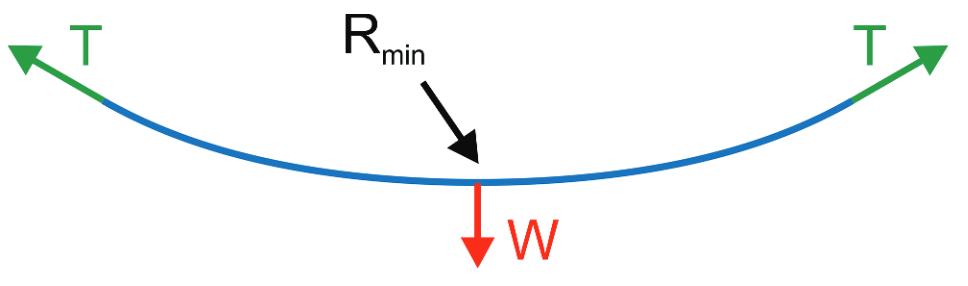
\includegraphics[width=0.3\textwidth]{p13.png}
    \caption{悬链线问题示意图\cite{nagyHighenergyFewcyclePulses2021}}\label{p4.4.1}
\end{figure}

长度为 l 的悬链线采用以下函数描述的形式：
\begin{equation}
    y=R_{\min}\cosh(x/R_{\min})
    \label{eq:4.4.1}
\end{equation}
其中，x和y分别表示水平和竖直方向的坐标，$R_{\min}$是位于曲线中间的最小曲率半径。

可以看出，$R_{\min} =\frac{T}{w}$ 是拉伸力与链条单位长度重量的比值（$w=\frac{W}{l}$）。因此，拉伸柔性空心光纤（SFHCF）的最小曲率半径可以通过增加拉伸力来优化，这使得这种毛细管几乎可以自由伸缩。由于壁厚较小，毛细管的比重通常小于 1 g/m。因此，只需要施加适当拉伸力，很容易能实现数公里量级的最小曲率半径。

\begin{figure}[h]
    \centering
    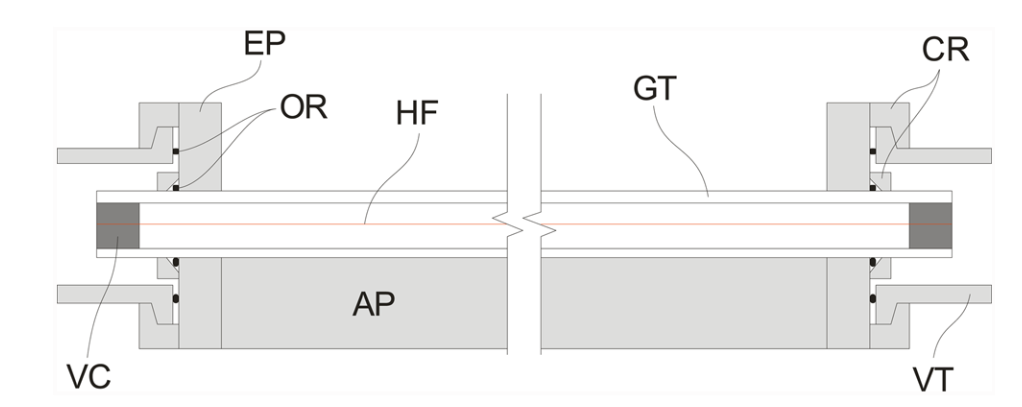
\includegraphics[width=0.4\textwidth]{p14.png}
    \caption{SFHCF测试组件。 HF：中空纤维； GT：玻璃管； VC：真空密封水泥； AP：配套铝型材； EP：端板； OR：O 形圈； CR：夹紧环； VT：真空管。\cite{nagyFlexibleHollowFiber2008}}\label{p4.4.2}
\end{figure}

为了确定新型中空光纤（见图 \ref{p4.3.1}（b））的波导特性，Tamas Nagy等人建造了一个 3 m 长的组件如图\ref{p4.4.2}。将氦氖激光器的几乎完美的衍射极限光束发射到 2.5 m 长的 SF-HCF 中。通过光电二极管测量波导的透射率，结果表明波导的透射率接近理论值，误差在1\%以内。此外，从光纤发出的光束在距离光纤端部一定距离处被记录，表现出完美的圆形光束轮廓，其发散度与数值计算值相匹配，如图 \ref{p4.4.3} 所示。这证明 SF-HCF 的输出光束实际上是衍射极限的。

\begin{figure}[h]
    \centering
    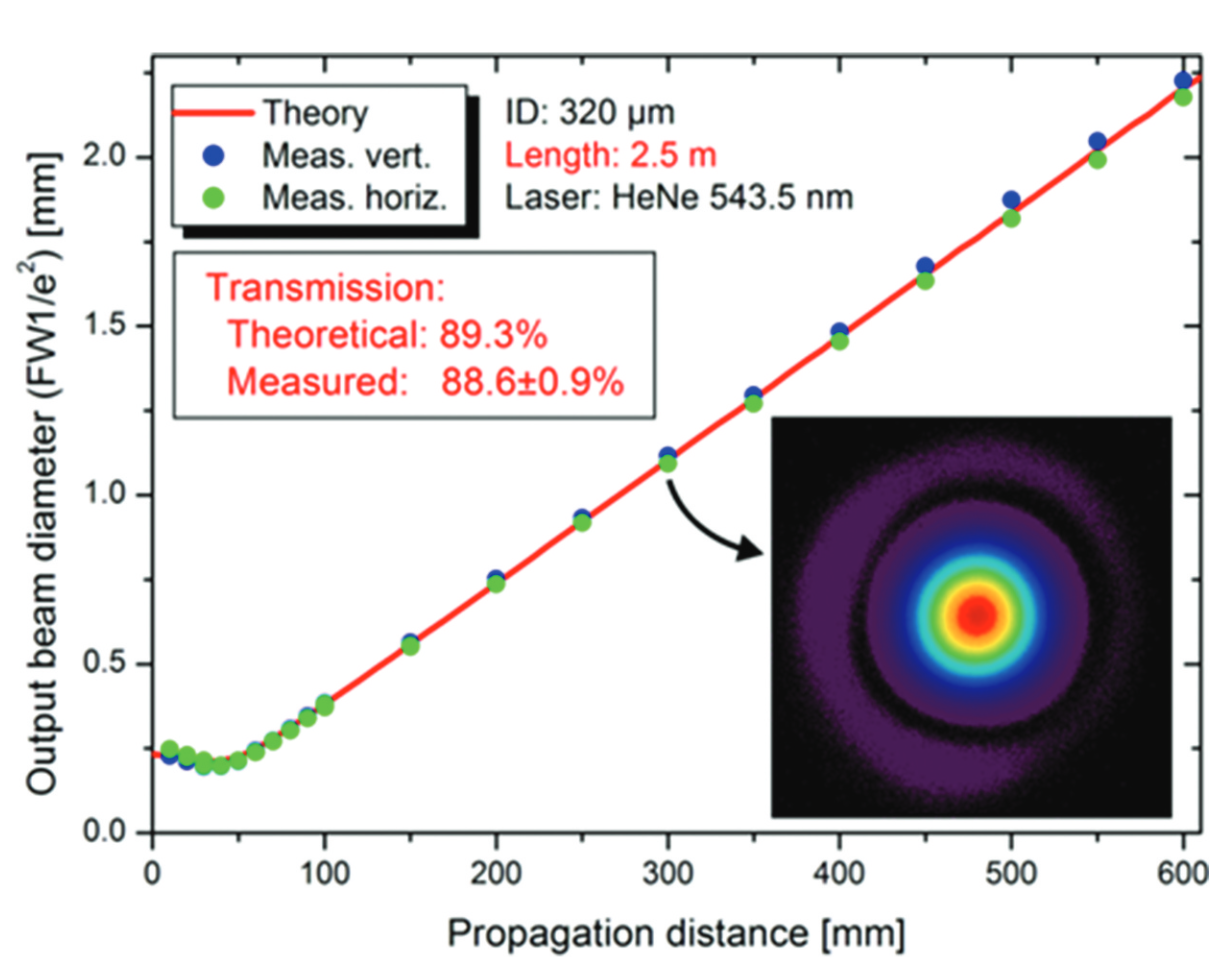
\includegraphics[width=0.3\textwidth]{p15.png}
    \caption{SF-HCF 的波导特性\cite{nagyFlexibleHollowFiber2008}}\label{p4.4.3}
\end{figure}

由于其具有自由的长度可扩展性以及接近理想的波导特性，SF-HCF 现已成为在严苛的压缩任务中采用的第二代中空光纤。事实上，迄今后压缩技术的大部分记录都是由 SF-HCF 取得的。

\subsection{进一步扩展的技术：压力梯度、电离、平面波导、多路复用和分子气体}

\subsubsection{压力梯度气体光谱展宽}

4.1节中描述的缩放定律描述的是单纯基于克尔效应的光谱展宽。作为压缩器设计的一般准则通常非常有用，但同时其也要求了很长的几何形状通常难以构建。人们开发了多种方法“过度驱动”光谱展宽过程从而进一步扩展基于波导的后压缩器的范围。这些技术总是在可实现的光谱展宽、峰值功率和多模操作之间进行仔细的权衡。

其中一项最为强大的技术之一，具有压力梯度的中空光纤，由 K. Midorikawa 团队引入，实验配置由图\ref{p4.5.1}所示。为减轻可能发生成丝的高强度的区域中气体介质的严重耦合损耗，A. Suda 和其同事将 HCF 两端的气体体积分离，光输入端的压力最小，输出端的压力较高。\cite{sudaGenerationSub10fs5mJoptical2005}

\begin{figure}[h]
    \centering
    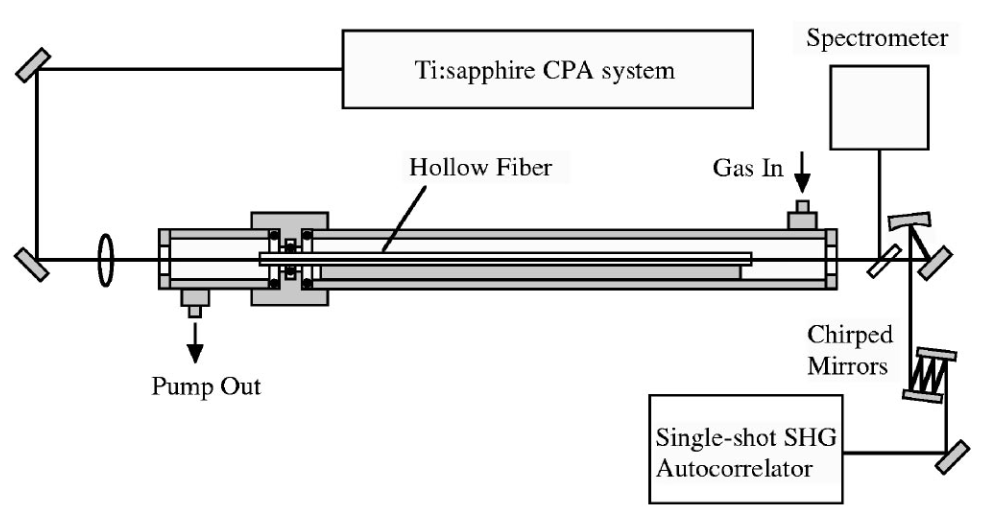
\includegraphics[width=0.5\textwidth]{p16.png}
    \caption{K. Midorikawa 团队压力梯度中空光纤实验配置\cite{sudaGenerationSub10fs5mJoptical2005}}\label{p4.5.1}
\end{figure}

从光输出侧提供的气体穿过光纤流向输入端，从而在光纤内部产生压力梯度，通过这种方式，可以在高强度下保持最佳的耦合，从而防止光纤前面的成丝引起的光束重塑。由于纤维内部的压力梯度，不可压缩粘性流体的压力分布如下：
\begin{equation}
    p(z)=\sqrt{p_0^2+\frac zL\left(p_L^2-p_0^2\right)}
    \label{eq:4.5.1}
\end{equation}
其中 $p_0$ 和 $p_L$ 是长度为 L 的毛细管前后的气压，实验中使用。

与恒定气压的传统方法相比，有几个优点：

（1）通过降低该端的压力可以避免不利的非线性现象，例如光纤入口周围的自聚焦和成丝。

（2）入射光束与最低阶光纤模式良好耦合后，在传播过程中逐渐与气体介质相互作用，进行自相位调制。

（3）由于光纤内部光损耗而导致的传播过程中非线性的降低在一定程度上被压力梯度所补偿。

（4）通过这种方案，非线性相互作用逐渐建立，延迟了光纤内部的自聚焦和电离，从而抑制了高阶本征模的数量。 

该方法的缺点是有效相互作用长度减少 $L_{\mathrm{eff}}\approx\frac{2}{3}L$。这个问题可通过使用长波导缓解，正如我们对标准 HCF 与长 SF-HCF 性能的比较研究所证明的那样，\cite{nagyOptimalPulseCompression2011}其结构支持压力梯度操作。

后来，Nam 的团队在 1 m 长、300 $\mathrm{\mu m}$ 内径的 HCF 中，用氖气 C.H. 进行差动泵送，在 0.2 TW 下产生了 5.5 fs 脉冲，后来在 0.3 TW 峰值功率下产生了 3.7 fs 脉冲。这些研究高达 1.2 mJ 的压缩脉冲能量受到可用中空光纤长度（1 m）的限制。

K.Midorikawa的小组在内径为500 $\mathrm{\mu m}$、长2.2 m充氦HCF中使用压力梯度，将钛宝石激光器脉冲首先压缩到低于10 fs\cite{sudaGenerationSub10fs5mJoptical2005, oishiSub10FsMultimillijoule2005}，然后压缩到具有多mJ能量的2周期持续时间\cite{bohmanGenerationFsTW2008}，最终形成了5 mJ、5 fs脉冲这一长期记录。
 
对于少数周期脉冲，稳定并控制其载波包络相位（CEP）非常重要。因此要证明使用压力梯度的HCF内的层流气流不会降低脉冲的CEP稳定性\cite{okellCarrierenvelopePhaseStability2013, luckingSituMeasurementNonlinear2014}。此外在HCF中，通过压力梯度良好控制的内耦合可以对高能脉冲的傅立叶变换极限持续时间进行简单的压力调节\cite{robinsonGenerationIntenseTransformlimited2006}。

综合上述提高能量范围的方法：
 
 （i）使用氦气；
 
 （ii）圆偏振光；
 
 （iii）大孔径的长毛细管；
 
 （iv）压力梯度。

Marie Ouillé等人与R.Lopez-Martens团队合作，通过压缩8 mJ 23 fs脉冲，在孔径为450 $\mathrm{\mu m}$、长2 m的SF-HCF中实现了CEP稳定的3 mJ，4 fs脉冲，配置图如图\ref{p4.5.2}所示。\cite{ouilleRelativisticintensityNearsinglecycleLight2020}
 
\begin{figure}[h]
    \centering
    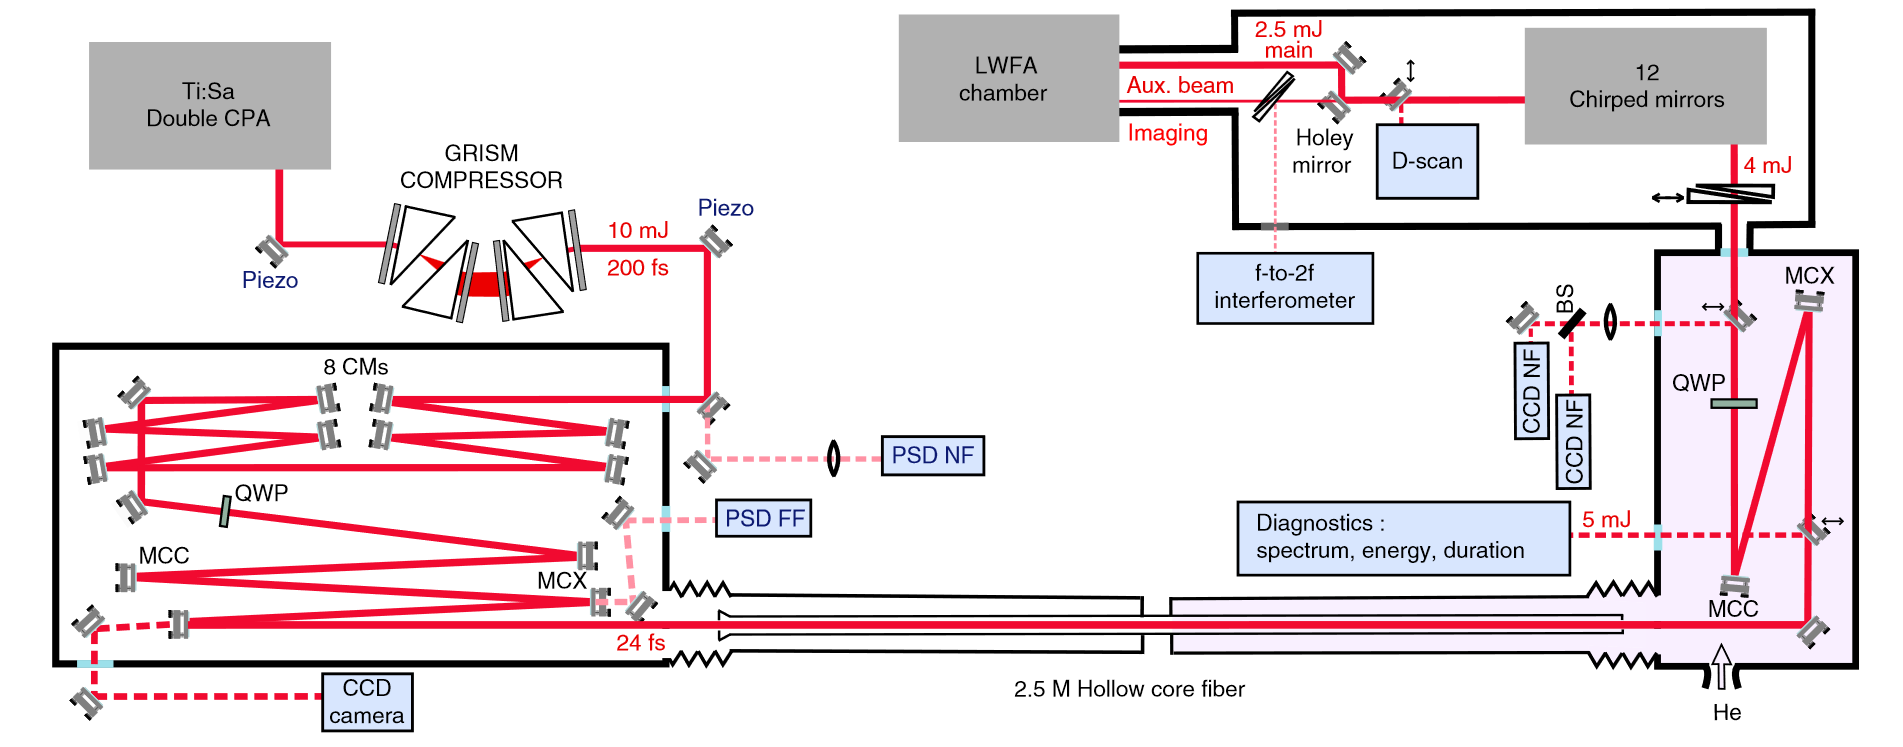
\includegraphics[width=0.9\textwidth]{p17.png}
    \caption{Marie Ouillé 等人真空集成拉伸柔性中空纤维脉冲压缩机装置示意图。PSD：光敏探测器、NF：近场、FF：远场、piezo：压电驱动镜座、MCX：凸面镜、MCC：凹面镜、QWP：四分之一波片\cite{ouilleRelativisticintensityNearsinglecycleLight2020}}\label{p4.5.2}
\end{figure}

在这项研究中，Nagy Tamas等人发现：HCF组件的输入窗口内的过度非线性（B>3 rad）会导致内耦合恶化，从而导致波导的传输恶化，而波导的传输无法通过纵向移动光纤入口来恢复。因此，由于可用于压缩机的总长度被严格限制在5.5 m，进一步将系统的输入能量增加到10mJ需要构建具有集成HCF的真空束线。在当前设置中，所有聚焦/再准直光学器件都位于真空/气体室中，并且只有低强度的大准直光束通过窗口而不会引起不希望的非线性。通过这种方式，常规生成具有3.5 mJ的良好控制的CEP稳定的3.5 fs脉冲。
 
最近，该系统的放大版已在Max Born研究所投入使用，总长度为8.2 m，其中14 mJ 50 fs脉冲被压缩为1.5个光学周期，持续时间为3.8 fs，输出能量为6.1 mJ，峰值功率为1.2 TW打破了TW大关。\cite{nagyGenerationAboveterawatt5cycle2020}

\subsubsection{电离实现光谱展宽}

在更高的输入峰值功率和脉冲能量（TW级输入脉冲）下，可以利用光电离诱导的相位调制，而不是Kerr效应。基于这种相位调制机制，小组在低压充氦HCF中以10 Hz的重复频率将~70 mJ、40 fs的脉冲压缩到11 fs，能量为13.7 mJ。\cite{dutinPostcompressionHighenergyFemtosecond2010, augusteApplicationOpticalfieldionizationinducedSpectral2012, augusteHighenergyFemtosecondLaser2013}在后来的工作中，他们以8.7 mJ的能量获得了9 fs的脉冲\cite{hortPostcompressionHighenergyTerawattlevel2015}。

然而，该技术面临高损耗和长的压缩脉冲持续时间的问题。

\subsubsection{平面波导（PWG）光谱展宽}

还有一种替代的解决方案：通过更大尺寸的波导来大幅增加模式面积代替毛细管，如中空平面波导（PWG）（如图\ref{p4.5.3}）。K.Midorikawa的小组将一组PWG安装在长度为1.9 m的气室中心，使用氩气作为非线性介质在适度压力下光谱增宽，获得了2mJ，12fs的脉冲。\cite{nurhudaOpticalPulseCompression2006, chenCompressionIntenseUltrashort2008}

\begin{figure}[h]
     \centering
     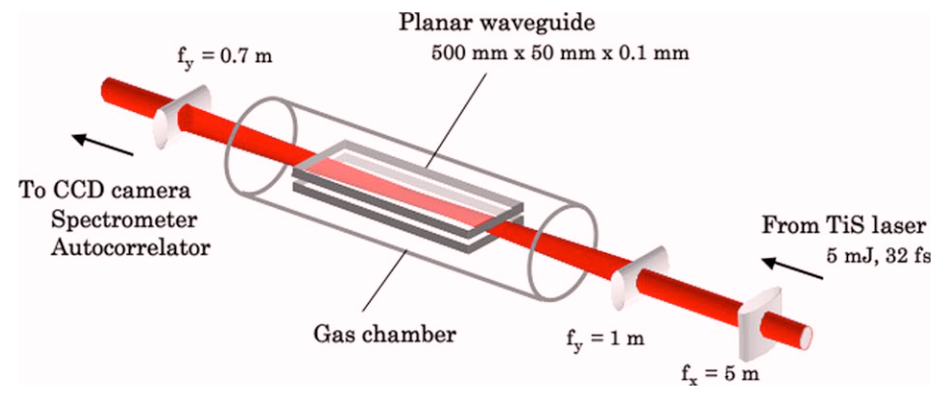
\includegraphics[width=0.5\textwidth]{p18.png}
     \caption{K.Midorikawa的小组中空平面波导压缩系统的几何结构示意图\cite{nurhudaOpticalPulseCompression2006, chenCompressionIntenseUltrashort2008}}\label{p4.5.3}
\end{figure}
 
A.Mysyrowicz的团队分析并改进了这项技术，使用空心锥形PWG（tPWG）如图\ref{p4.5.4}所示，这种锥形配置具有将高输出功率与先前在传统PWG中不容易获得的高光束质量相结合的优点，最终在10–12 fs的持续时间内达到约10 mJ的脉冲能量。\cite{chenCompressionHighenergyUltrashort2011}

\begin{figure}[h]
    \centering
    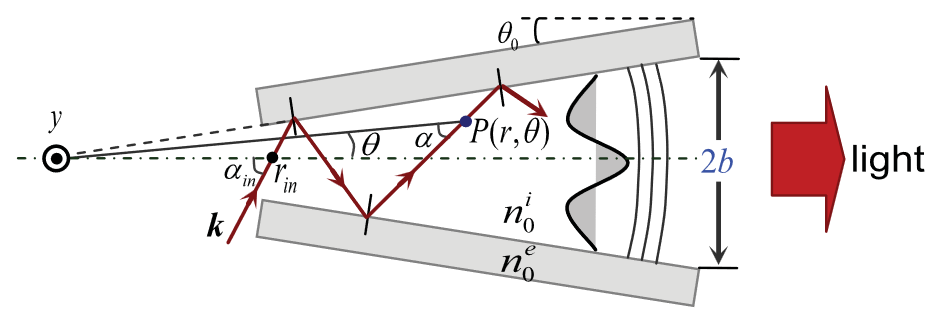
\includegraphics[width=0.5\textwidth]{p19.png}
    \caption{由两个略微倾斜的抛光熔融二氧化硅板组成的空心锥形PWG配置示意图\cite{chenCompressionHighenergyUltrashort2011}}\label{p4.5.4}
\end{figure}

后来，C.Arnold小组在低于15 fs的持续时间内达到了太瓦水平，但自此这种方法就没有进一步的应用。

该技术的主要障碍与装置的不完整波导特性有关，因为没有平行于板的波导。因此，光束轮廓不能被控制在沿着这个方向上，导致不均匀的光谱增宽，并且在更高的强度下呈现多丝状态。

\subsubsection{多路复用方法/分脉冲非线性压缩（DPNLC）}

J.Limpert和P.Georges小组从分脉冲放大（DPA）中得到启发，提出了分脉冲非线性压缩的方法，如图\ref{p4.5.5}，将输入脉冲在进入HCF前分为具N个能量 1/N 的相同脉冲序列，每个脉冲独立地展宽。随后，脉冲被重新组合形成展宽光谱的高能脉冲\cite{klenkeDividedpulseNonlinearCompression2013, guichardEnergyScalingNonlinear2013}。

\begin{figure}[h]
    \centering
    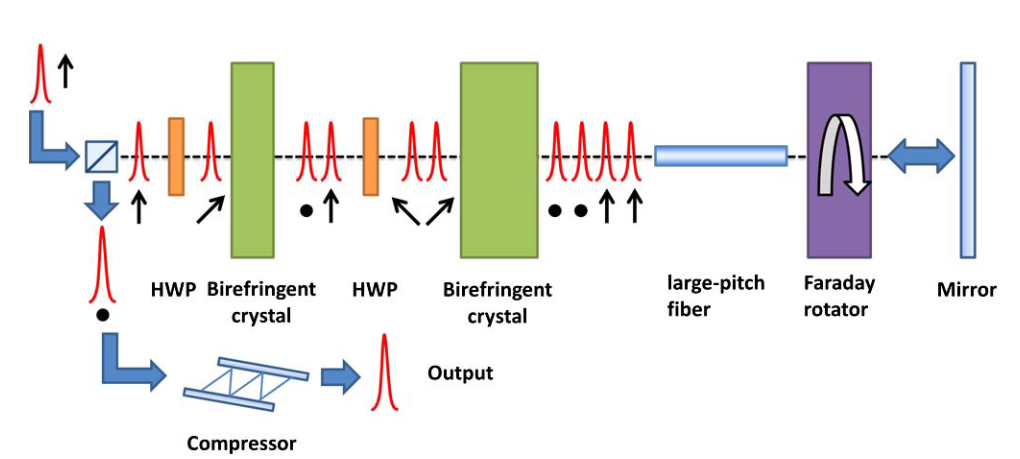
\includegraphics[width=0.6\textwidth]{p20.png}
    \caption{时间分脉冲非线性压缩实验装置\cite{klenkeDividedpulseNonlinearCompression2013}}\label{p4.5.5}
\end{figure}

双折射晶体已用于DPA方法，以从飞秒或皮秒脉冲创建脉冲复制品（图\ref{p4.5.5}）。通过慢轴和快轴之间折射率的不同，在时间上分离线偏输入脉冲的正交偏振分量。通过不同长度的几种晶体与半波片（HWP）交替的组合最终产生所需的脉冲串。最终，通过法拉第旋转器将整个脉冲串的偏振态翻转90°，并在相反方向上通过相同的晶体序列再次传播回来，消除了时间延迟。


这种多路复用方法对于具有窄频谱的较长脉冲表现良好；然而，由于缺乏宽带无色散偏振分束器和组合器，将其应用于少数周期脉冲并非易事。R.Lopez-Martens的小组利用晶体中的双折射进行分裂和复合，将这种方法应用于少循环状态。\cite{jacqminPassiveCoherentCombining2015, jacqminTemporalPulseDivision2015}

\begin{figure}[h]
    \centering
    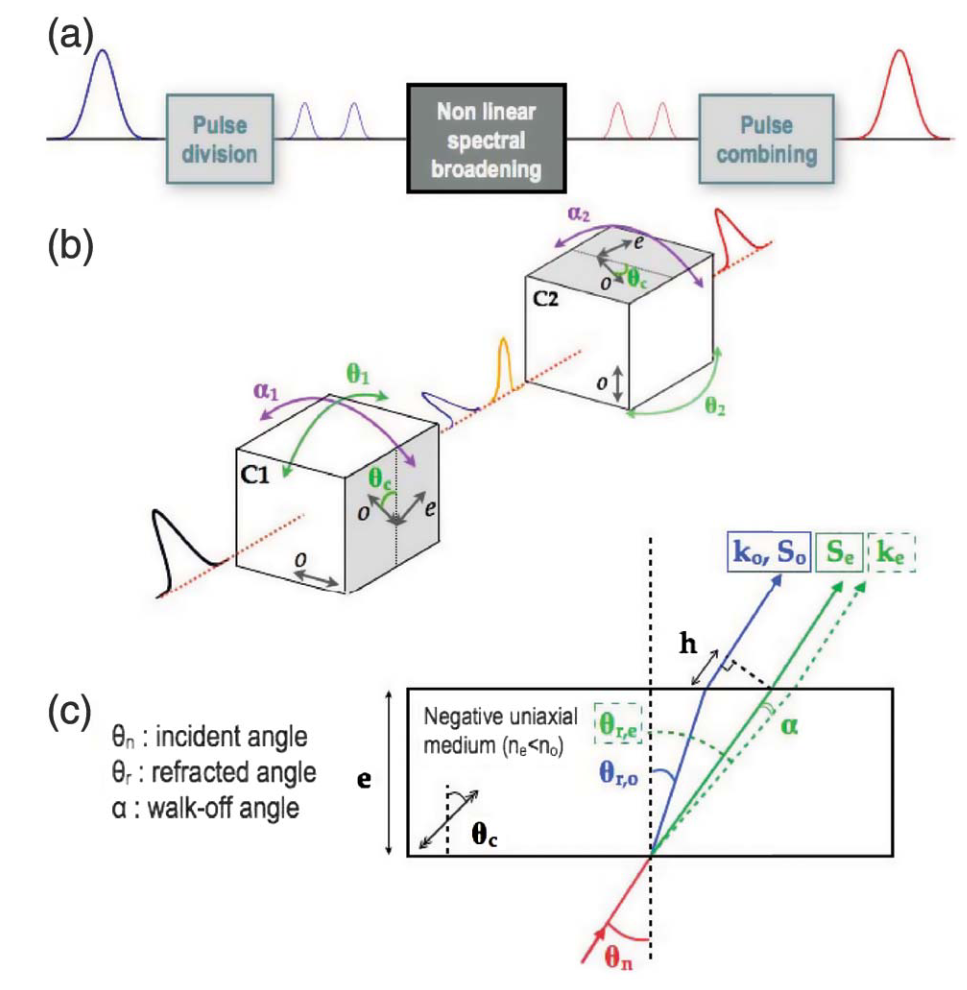
\includegraphics[width=0.4\textwidth]{p21.png}
    \caption{R.Lopez-Martens的小组（a） 分脉冲非线性压缩示意图。（b） 方解石板块的方向。（c） 第二个双折射板的俯视图：普通（蓝色）和非寻常（绿色）光线。\cite{jacqminTemporalPulseDivision2015}}\label{p4.5.6}
\end{figure}

类似于时间复用方案，也可以使用空间复用在分离的HCF中对分割的脉冲进行频谱扩展，然后再进行重组。光束的偏振用半波片旋转，如下偏振分束器立方体（PBS）将其分为两个具有相等功率的子光束。一个耦合到光纤1中，另一个通过四分之一波片和压电驱动反射镜组成的延迟线。这种组合使偏振旋转90度。因此，光束通过分束器并耦合到增宽光纤2中。两个光束使用第二个PBS组合。组合光束的功率与两入射光束间相位差无关。然而，偏振态根据该相位差在线性偏振和椭圆偏振间变化。为了优化组合光为线偏振，一小部分功率被反射到Hänsch–Couillaud探测器\cite{hanschLASERFREQUENCYSTABILIZATION1980}（图中的HC）。该检测器可以使用组合光束的偏振状态来估计两个光束之间的相位差。生成的误差信号通过PID调节器反馈到延迟线中的压电驱动反射镜。稳定系统的带宽约为1kHz，受压电安装反射镜的限制。\cite{klenkeCoherentCombinationSpectrally2014}

\begin{figure}[h]
    \centering
    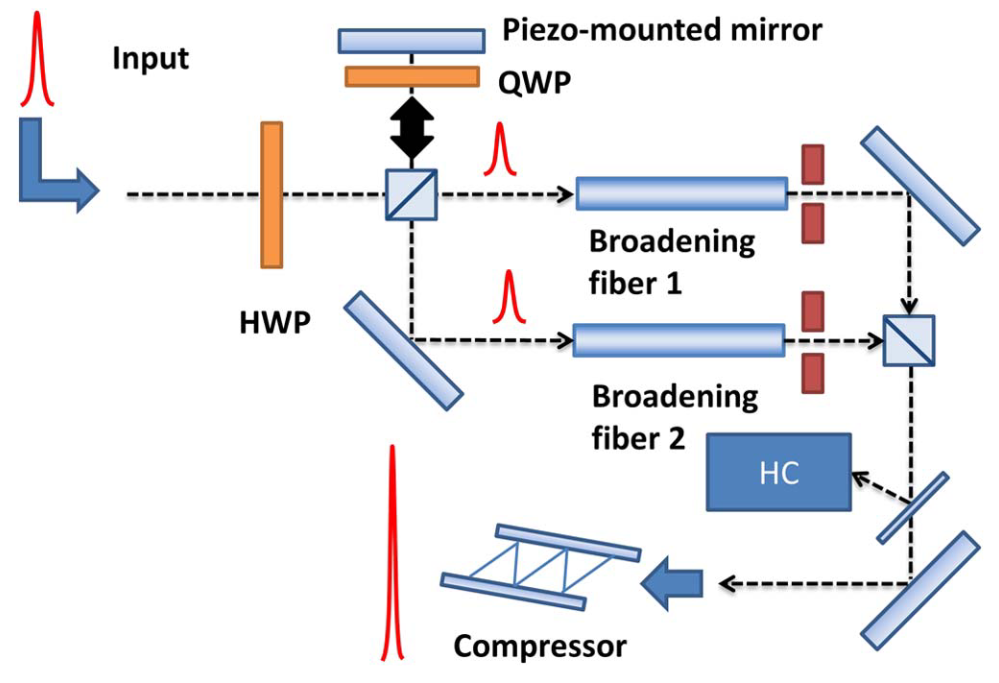
\includegraphics[width=0.4\textwidth]{p22.png}
    \caption{空间复用实验示意图。HWP，半波片；QWP，四分之一波片；HC，Hänsch–Couillaud探测器。\cite{klenkeCoherentCombinationSpectrally2014}}\label{p4.5.7}
\end{figure}

\subsubsection{分子气体}

有些情形需要将HCF缩放按相反的方向进行：脉冲能量低或脉冲持续时间长，峰值功率不足以使用充满惰性气体的HCF进行光谱展宽。这种情况下，分子气体提供了一种解决方案：分子旋转（拉曼散射）引起非瞬时非线性响应，导致光谱的红色侧显著增强。

分子气体优点：

（1）这种缓慢的非线性效应可能比瞬时的克尔效应大得多，使其适合低峰值功率脉冲的压缩，但输入脉冲持续时间需要足够长以经历拉曼效应（>100fs）；

（2）许多分子气体相对于原子气体，非线性和电离势之间的比例通常更好，导致更大的光谱展宽能力；\cite{haddadMolecularGasesPulse2018, fanHighEnergyRedshifted2020}

（3）通过将输入脉冲持续时间与延迟非线性的时间常数适当匹配（或为输入脉冲找到合适量），可极大地优化光谱增宽和线性调频；

J.E.Beetar等人最近发表的一篇文章所示。[173]实现了45倍压缩和两个倍频程跨度的光谱。该技术非常适合于Yb基激光器的几个100fs长脉冲的压缩。


然而，分子运动摩擦产生的热量可能会限制使用分子气体的平均功率缩放，使其是否适用于功率为瓦特量级、10 s或100 s的高重复率系统尚有疑问。

\section{自压缩技术}

除了使用光谱展宽和随后的压缩步骤组成的后压缩技术外，还有另一种方法，即在非线性传播过程中利用自压缩动力学。

这些技术有很大前景，可实现最短的光脉冲（不包括高次谐波产生，这是一个二次过程），直至具有多倍频的子周期范围，远远超出当今啁啾补偿技术的能力。

不利方面，由于依赖于对输入脉冲参数非常敏感的高度非线性动力学，很难缩放脉冲能量和峰值功率。如今，只有中红外光谱范围内的驱动脉冲，通过自压缩技术产生的很少周期脉冲可以超过mJ水平。此外，自压缩脉冲通常在脉冲的前沿表现出相当长的基座。

H.C.Kapteyn和M.M.Murnane小组开创性地在充满低压氩气的短空心波导中，观察到电离主导传播过程中的自压缩，通过将2.2 mJ 30 fs的Ti:蓝宝石脉冲耦合到内径为150 $\mathrm{\mu m}$的2.5 cm长的HCF中，获得了13 fs的脉冲。\cite{wagnerSelfCompressionUltrashortPulses2004}

自压缩也可在成丝过程中，基于自聚焦、电离诱导的散焦、SPM以及自陡化之间的复杂相互作用获得。Sergei A. Trushin等人通过在差分真空级中突然去除非线性介质而终止成丝后，可直接在光丝内部观察到自压缩至11fs。\cite{trushinSub10fsSupercontinuumRadiation2007}使用类似技术如图\ref{p5.0.1}，Emilia Schulz首先依赖于半无限气室（SIGC）双差分泵送方案来实现高压梯度，SIGC中的大气压下能够实现丝状，而向真空的急剧转变确保了脉冲的所有非线性效应的突然结束。通过扫描灯丝的真空跃迁，提取并分析了来自非线性相互作用区不同位置的红外脉冲通过光谱仪跟踪脉冲沿光丝的演变。\cite{schulzTrackingSpectralShapes2011}

\begin{figure}[h]
    \centering
    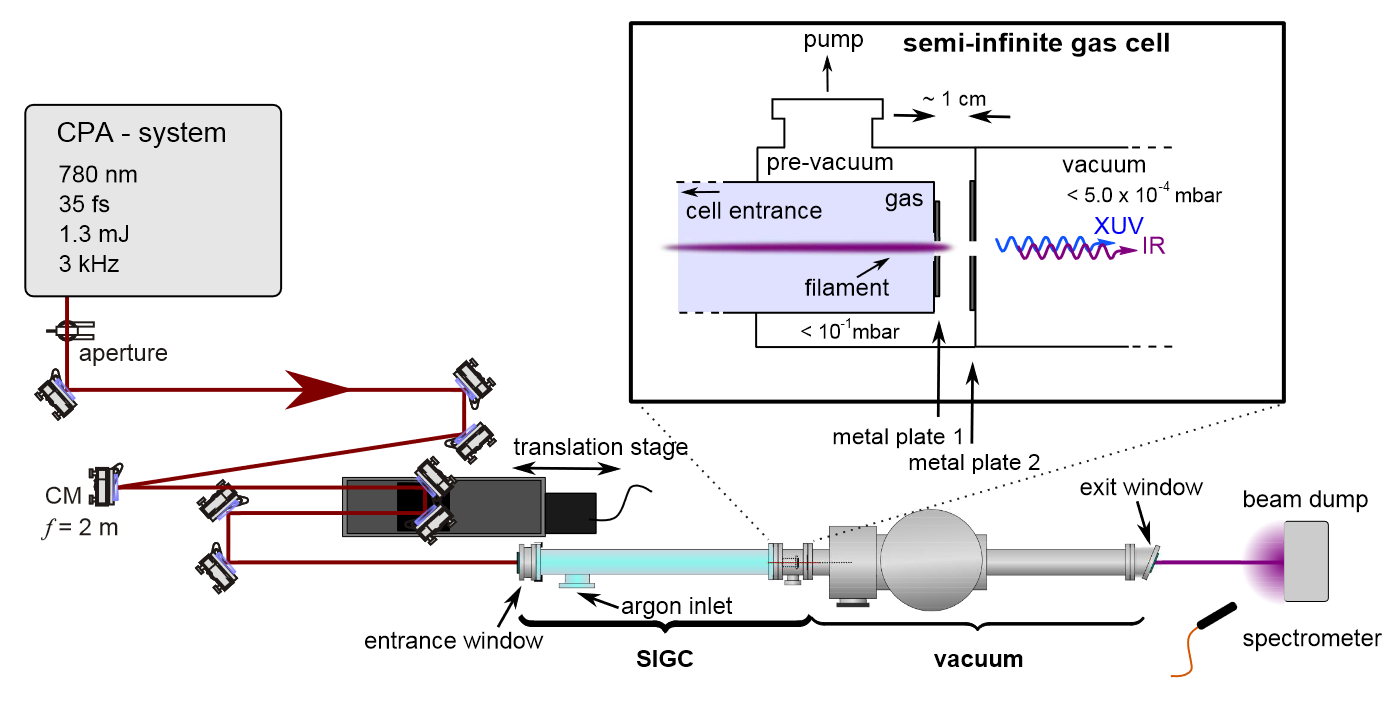
\includegraphics[width=0.65\textwidth]{p23.png}
    \caption{Emilia Schulz实验设置：来自啁啾脉冲放大器的脉冲由曲面镜（CM）聚焦到充满氩气的半无限气室（SIGC）中。在氩气中形成光丝被针孔截断，随后在真空中传播。所产生的白光与出射窗口耦合，用于光谱分析。\cite{schulzTrackingSpectralShapes2011}}\label{p5.0.1}
\end{figure}

\begin{figure}[h]
    \centering
    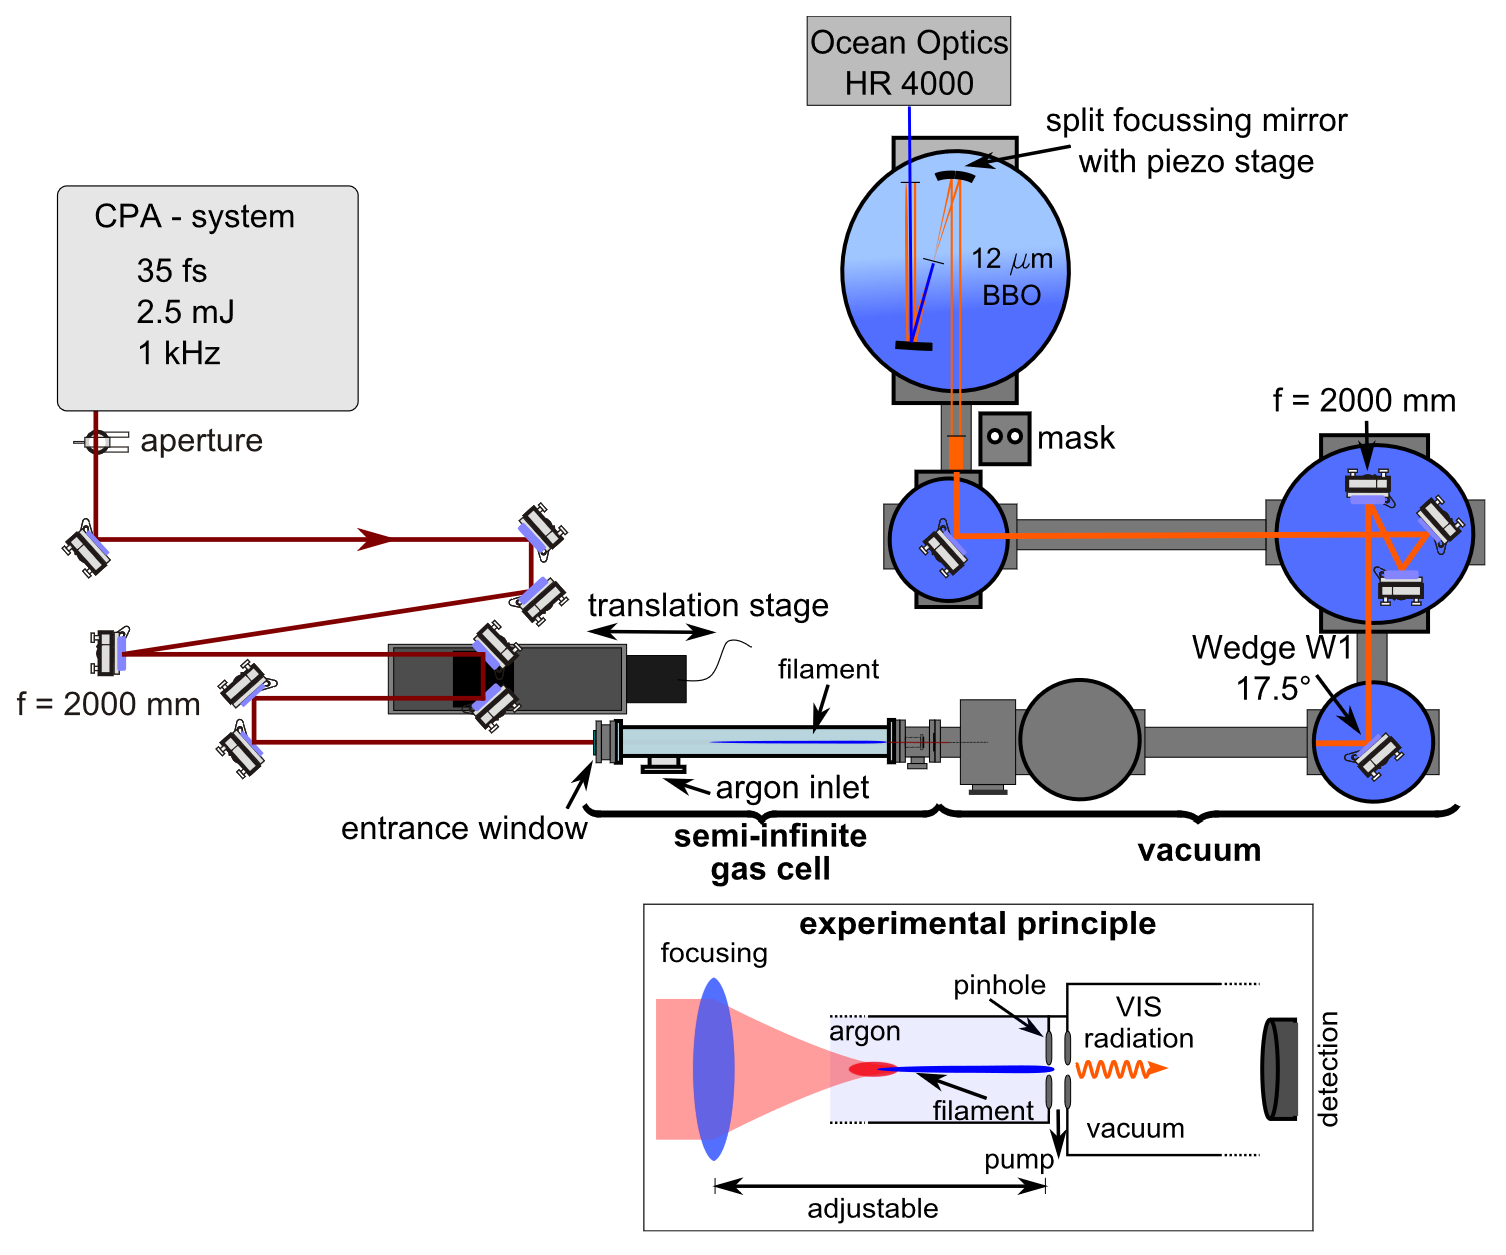
\includegraphics[width=0.5\textwidth]{p24.png}
    \caption{实验装置示意图：通过SHG-FROG设置，在随后的全真空室中直接表征出现的脉冲，从而能够对基本脉冲形状进行不受干扰的观察。\cite{kretschmarDirectObservationPulse2014}}\label{p5.0.2}
\end{figure}
Martin Kretschmar等人随后通过放置在光丝后面真空中的FROG设备跟踪脉冲沿细丝的演变，如图，揭示了丰富的时空动力学，导致形成持续时间为5 fs的更短脉冲\cite{kretschmarDirectObservationPulse2014}。



\begin{figure}[htbp]
    \centering   %居中放置
    \subfigure[光谱与变换极限脉冲时间演化] %为每个图片加上编号
    {
        \begin{minipage}[b]{.4\linewidth} %表示在该行所占空间的比例为0.3；其中。3=0.3；b为放置方式；
            \centering
            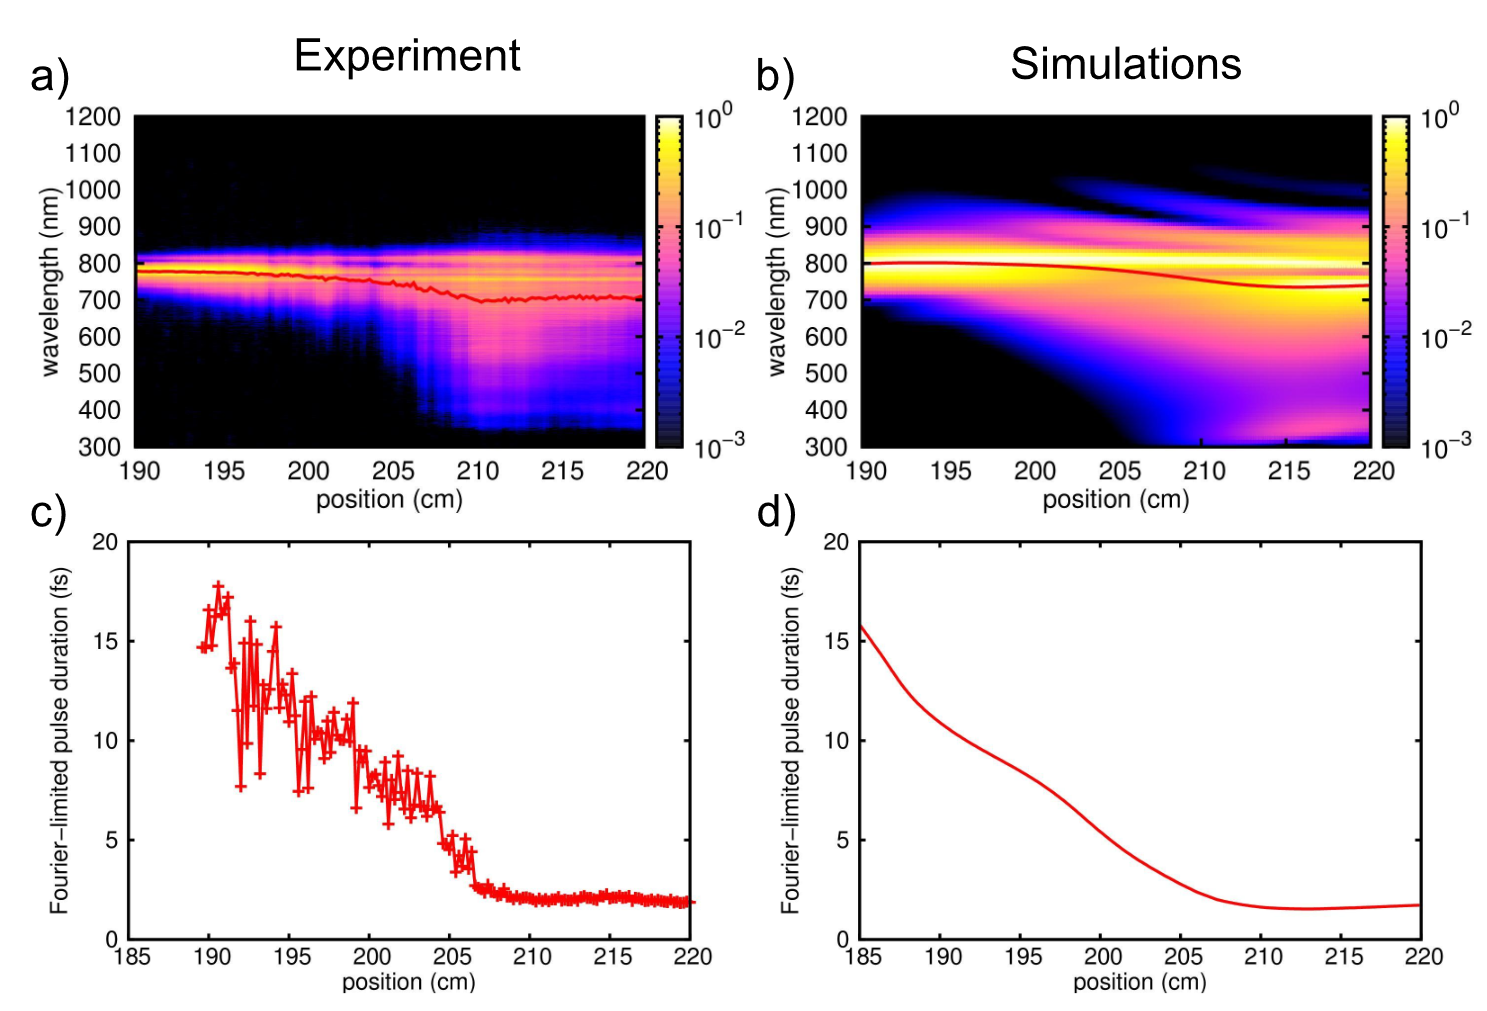
\includegraphics[scale=0.13]{p25.png}
        \end{minipage}
    }
    \subfigure[FROG测量脉冲形状演化]
    {
        \begin{minipage}[b]{.4\linewidth}
            \centering
            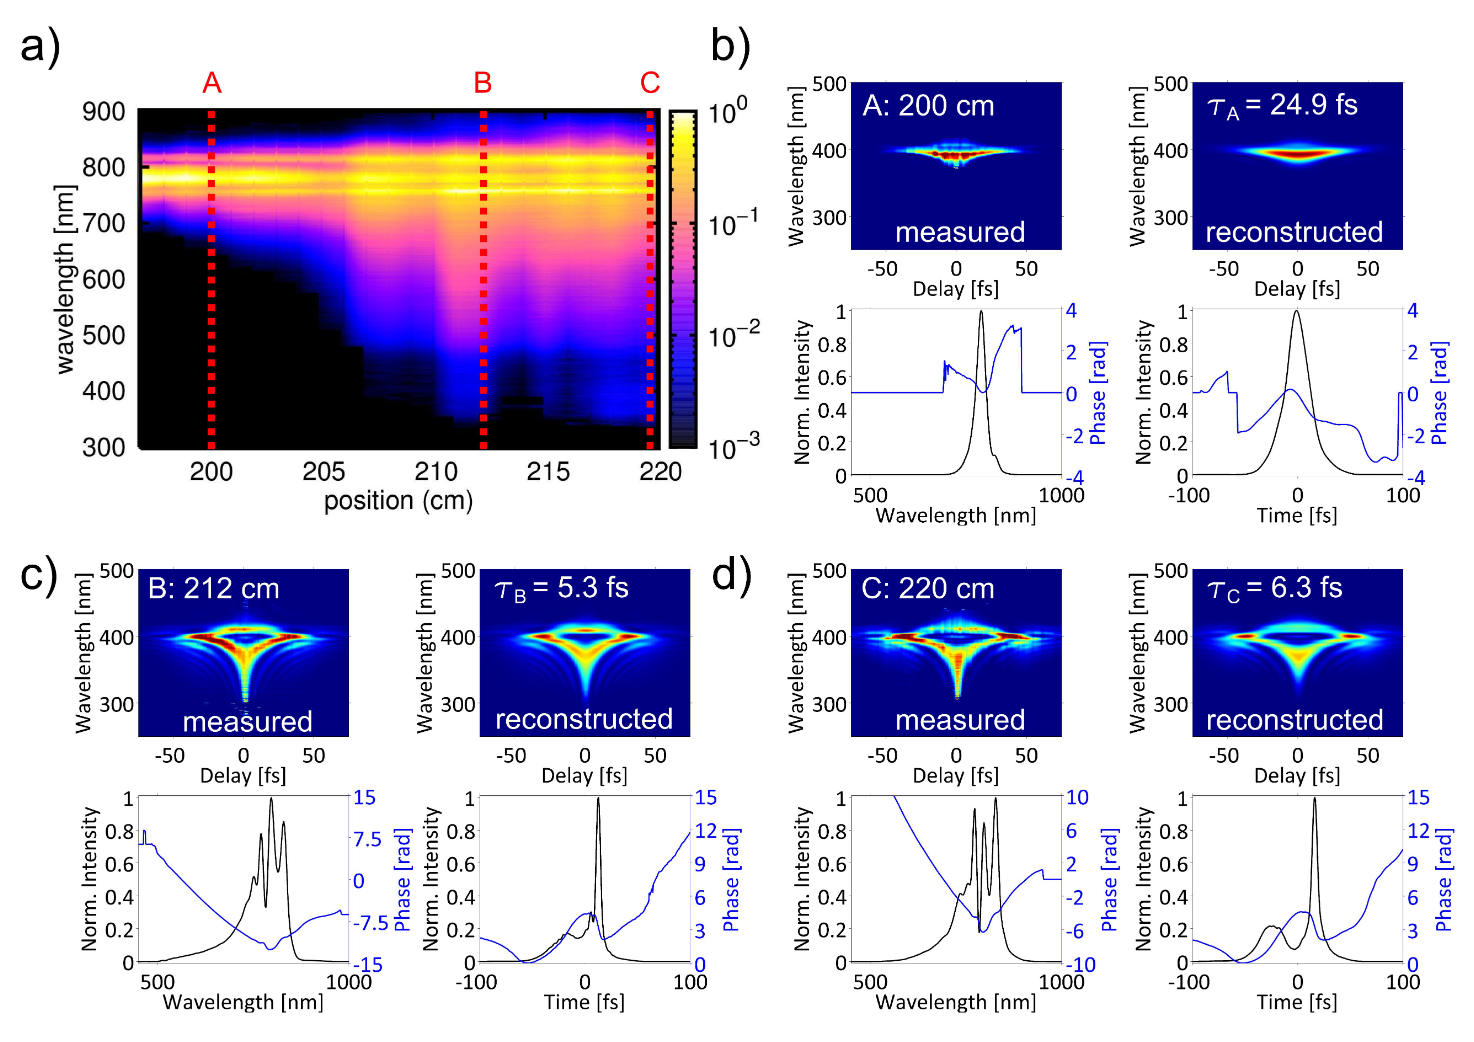
\includegraphics[scale=0.13]{p26.png}
        \end{minipage}
    }
    \caption{光丝传播过程中光谱与脉冲形状变化}
\end{figure}

在中红外波段，大多数材料都表现出异常色散，这与克尔效应相结合，也会导致孤子传播引起的压缩。最近也使用包含熔融二氧化硅板作为1550 nm非线性介质的多通腔证明了这一点\cite{jargotSelfcompressionMultipassCell2018}。在这个光谱范围内发生成丝情况下，很难清楚地确定成丝动力学或孤子传播在自压缩中占主导地位。

在3.9μm波长下的实验——在大块YAG板中观察到的21 mJ 94 fs脉冲到30 fs的自压缩\cite{shumakovaMultimillijouleFewcycleMidinfrared2016}，以及后来在氮气中正啁啾18mJ、100fs脉冲被压缩到16mJ能量下的39fs，根据孤子传播进行了解释\cite{shumakovaMultimillijouleFewcycleMidinfrared2016}。在另一个具有相同光源的实验中，实现了对29.5 mJ能量的正啁啾150 fs脉冲的自压缩，具有与前一种情况相似的峰值功率，在0.34 TW的峰值功率下被压缩到持续时间为28 fs的亚3周期，被解释为在空气丝中形成了光弹（在空间和时间上高度局部化的光包），如图\ref{p5.0.4}所示。\cite{shumakovaChirpcontrolledFilamentationFormation2019}。

\begin{figure}[h]
    \centering
    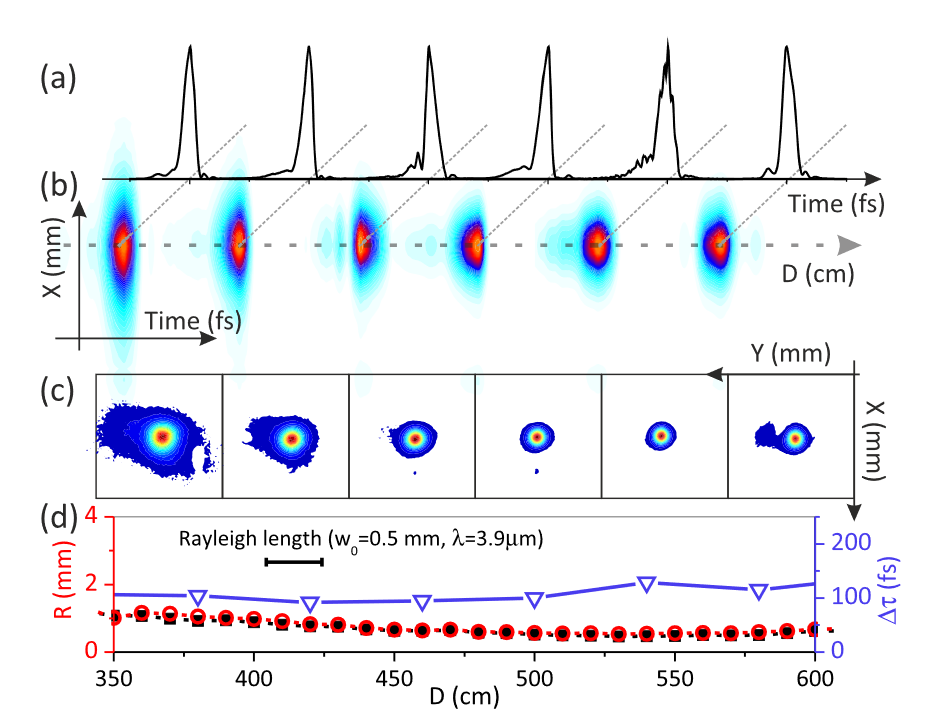
\includegraphics[width=0.5\textwidth]{p27.png}
    \caption{在持续时间为130fs的正啁啾脉冲的情况下，观察到沿着灯丝形成的光弹\cite{shumakovaChirpcontrolledFilamentationFormation2019}}\label{p5.0.4}
\end{figure}

通过在具有负色散的空心波导中形成高阶孤子，可在$\mathrm{\mu J}$ 能量量级实现良好控制的自压缩。J.Herrmann的小组从理论上表明，空心Kagome晶格PCFs在整个可见光和紫外光谱范围内表现出必要的传输带宽和负色散，以支持孤子传播\cite{imGuidingPropertiesDispersion2009}。此外，他们预测了通过谐振色散波（RDW）发射产生的高能超连续谱和亚10fs、UV-VUV脉冲，该发射可通过波导中的气体压力进行调节\cite{imHighpowerSolitoninducedSupercontinuum2010}。随后，P.St.J.Russell的小组通过实验证明了这两种效应\cite{jolyBrightSpatiallyCoherent2011}。产生的RDW脉冲在240–350 nm的范围内可调谐，后来扩展到120–200 nm\cite{ermolovSupercontinuumGenerationVacuum2015}，包含几十nJ的能量。还产生了跨越三个八度以上的宽超连续谱\cite{belliVacuumultravioletInfraredSupercontinuum2015}。后来，通过使用大芯单环HC-PCF，该小组成功实现了自压缩到单循环状态，在MHz重复率下将UV脉冲能量放大到μJ水平\cite{kottigEfficientSinglecyclePulse2020}，并证明了自压的CEP稳定性\cite{ermolovCarrierenvelopephasestableSolitonbasedPulse2019}。

在孤子压缩的情况下，使用更长的波长也有助于能量缩放。T.Balciunas等人在充氩的大芯Kagome晶格微结构光纤中以25 $\mathrm{\mu J}$的能量将波长为1.8 $\mathrm{\mu m}$的35 $\mathrm{\mu J}$、80 fs脉冲压缩到4.5 fs的子周期持续时间。\cite{balciunasStrongfieldDriverSinglecycle2015}在3.25 $\mathrm{\mu m}$的更长波长下，在9.6 W的高平均功率下产生了持续时间为14.5 fs的近单周期脉冲。\cite{eluHighAveragePower2017}

\begin{figure}[h]
    \centering
    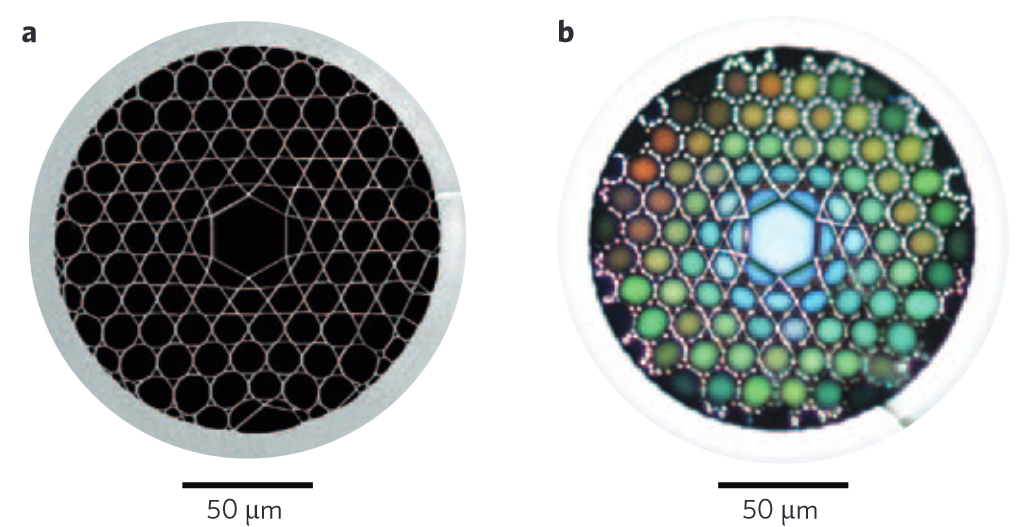
\includegraphics[width=0.5\textwidth]{p28.png}
    \caption{kagome型 HC-PCF\cite{russellHollowcorePhotonicCrystal2014}}\label{p5.0.5}
\end{figure}

J.C.Travers等人认识到，适当选择参数，充气毛细管也可表现出负色散，从而实现孤子动力学\cite{traversHighenergyPulseSelfcompression2019}。由于能量缩放需要几米长的高质量毛细管，因此他们的方法依赖SF-HCF。J.C.Travers的团队在内径为250 $\mathrm{\mu m}$的3米长充氦SF-HCF中，以100 $\mathrm{\mu J}$的能量将来自HCF压缩机的10 fs近红外脉冲压缩到亚fs持续时间。此外，如图\ref{p5.0.6}所示，通过改变气体压力，他们产生了高达16 $\mathrm{\mu J}$的脉冲能量可在120和350 nm之间调谐的少量循环UV脉冲。在最近的一项工作中，该小组使用具有反向压力梯度的波导解决了输出窗口的啁啾问题：在波导的入口处施加气体，并将输出侧置于真空中。\cite{brahmsResonantDispersiveWave2020}

\begin{figure}[h]
    \centering
    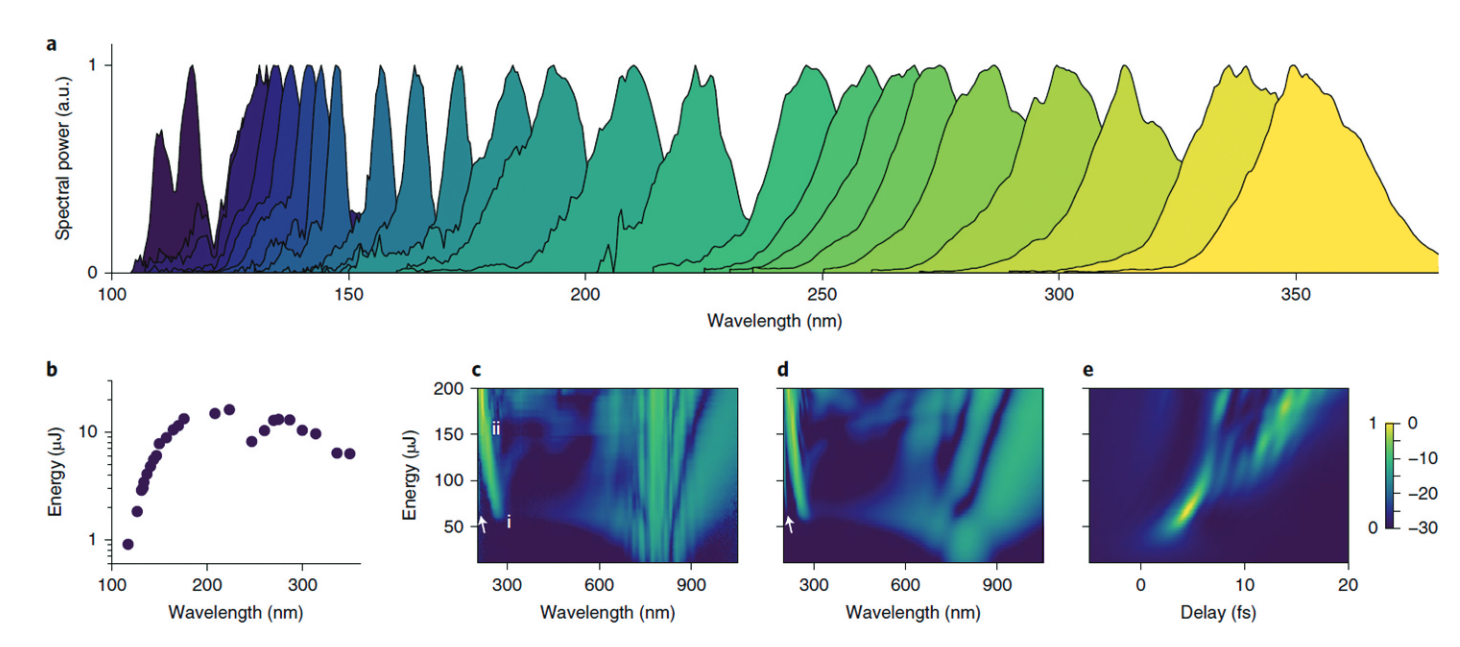
\includegraphics[width=0.9\textwidth]{p29.png}
    \caption{SF-HCF中孤子自压缩过程，通过谐振色散波发射在紫外范围内可调谐的少周期脉冲；（a） 测量的紫外线光谱，（b）脉冲能量。（c）HCF输出处的光谱演变（d）相应的模拟和（e）时间形状的模拟演变}\label{p5.0.6}
\end{figure}














%%%%%%%%%%%%%%%% 参考文献 %%%%%%%%%%%%%%%%%



\newpage

\clearpage           %%%  “目录”中显示的页码正确，需要添加 \clearpage
\phantomsection      %%   “目录”中的链接能正确跳转，需要添加 \phantomsection
\addcontentsline{toc}{section}{参考文献}   %向目录中添加条目，以章的名义

\bibliography{ref}

\end{document}